%!TEX TS-program = xelatex

\input{preamble/static}
\input{preamble/general}
\input{preamble/fonts}
\input{preamble/etc}

\addbibresource{bibliography/Bibliography.bib}

%Program * -> \cdot
\mathcode`\*="8000
{\catcode`\*\active\gdef*{\cdot}}

\begin{document}

\prefrontmatter
\calccentering{\unitlength}
\begin{titlingpage}
\thispagestyle{empty}
\sffamily
\vspace*{-2.8cm}
\hfill\includegraphics[scale=0.7]{DTU-logo-CMYK}
\begin{adjustwidth*}{\unitlength}{-\unitlength}
    \begin{adjustwidth}{-0.5cm}{-0.5cm}
		\noindent
		
		
		\vspace{\stretch{1}}
		\noindent\textbf{\Huge\ThTitle} \\*[0.2cm]
		\textcolor{dtured}{\rule{\textwidth + 1.5cm}{4pt}}
		\vspace{\stretch{1}} 
		\begin{flushleft}
		\Large
            \ThAuthors\\
            \thesistype{}\\
            \ThYear
        \end{flushleft}
		\vspace{\stretch{2}}
		\noindent
		\includegraphics[scale=0.26]{figures/IMG_0313_frontpage.png}
		\vspace{\stretch{1}}
		\newline
		\newline
		\newline
		%\noindent
		\includegraphics[]{tex_dtu_elektro_a_uk}
		%\vspace{-5cm}
	\end{adjustwidth}
\end{adjustwidth*}
	\cleartoevenpage
		\thispagestyle{empty}
		\ifnum\pdfstrcmp{\ThSubtitle}{}=0 %Check if there is a subtitle
		\noindent\textbf{\ThTitle}
		\else
		\noindent\textbf{\ThTitle, \ThSubtitle}
		\fi
		\vspace{\stretch{1}}

		\noindent\textbf{Report written by:}\\
		\ThAuthors

		\vspace{\stretch{2}}

		\noindent\textbf{Advisor(s):}\\
		\ThSupervisors

		\vspace{\stretch{3}}

		\noindent\ThDepartment

		\vspace{\stretch{4}}

		\noindent\ThElektroEmail

		\vspace{\stretch{5}}
		\frieze
		\noindent{\renewcommand{\arraystretch}{2}\begin{tabular}{@{}lp{0.75\textwidth}}
			Project period:&	\ThProjectPeriod\\
			ECTS:&		\ThECTS\\
			Education:&	\thesistypeabbr\\
			Field:&		\ThField\\
			Class:&		\ThClass\\
			Edition:&	\ThEdition\\
			Remarks:&	\ThRemarks\\
			Copyrights:&\ThCopyrights
		\end{tabular}}
		
\end{titlingpage}
\normalfont
\normalsize
\clearforchapter

\frontmatter
%!TEX root = ../Thesis.tex
\chapter{Abstract}
This thesis focuses on building, programming, and controlling a novel type of drone design. The drone behaves like a helicopter rotor as it rotates around its z-axis to create the lift necessary to keep it airborne. The focus is on finishing the drone's basic properties, such as assembling the foundation for a prototype, establishing sensor measurements, form communication between CPU and microcontrollers, and control the drone's rotation. The drone will need to have an estimate of its position in its rotation and be able to control its rotational velocity. The solution is implemented through two tasks: 1) calculating the drone's position with a fusion of sensor data, and 2) analyzing the system to implement a controller. The proposed solution shows that the drone estimates its position with high accuracy at low speeds, but lacks in sampling frequency to maintain this at high rotational velocities. The modeled system is shown to be very similar to the real drone. Finally, the drone is implemented with a PD-controller and feed-forward branch. The controller is successful in regulating the motors' voltage to maintain a specific angular velocity.
%!TEX root = ../Thesis.tex
\chapter{Preface}
This Bachelor's thesis was prepared at the Department of Electrical Engineering at the Technical University of Denmark in fulfillment of the requirements for acquiring a Bachelor of Science degree in Electrical Engineering.


\vfill

\iffalse
{
\centering
    \thesislocation{}, \today\\[1cm]
    %\hspace{3cm}\includegraphics[scale=0.4]{Signature}\\[1cm]
\begin{flushright}
    \thesisauthor{}
\end{flushright}
}
\fi
%!TEX root = ../Thesis.tex
\chapter{Acknowledgements}
We want to thank our advisor from DTU Elektro, Associate Professor Jens Christian Andersen, for excellent guidance during this project. Given COVID-19, we were unable to get into a lab for many weeks. He helped us borrow equipment to continue our development elsewhere and later on re-gained us access to the lab. Due to the fact that we inherited the project from our advisor, it was critical that he was available and able to help us get up to speed. \\
Jens Christian Andersen also assisted us a significant amount when we needed new and improved 3D printed parts and obtaining components for the project. 
\clearforchapter
\tableofcontents
\pagebreak
\listoffigures*
\listoftables*
\textbf{List of abbreviations and phrases}
\begin{itemize}
    \item RPM = Revolutions pr minute
    \item ESC = Electronic speed controller
    \item PWM = Pulse width modulation
    \item RPi = Raspberry Pi 
    \item AoA = Angle of attack
    \item IMU = Inertial measurement unit
    \item PCB = Printed circuit board
    \item ROM = Read-only memory
    \item EOL = End of line
    \item OS = Operating System
    \item DPS = Degrees per second
    \item mutex = mutual exclusion
    \item ISR = Interrupt service routine
    \item SysID = System Identificiation Toolbox
    \item SISO = Single input single output
    \item Li-PO = Lithium-ion polymer battery
    \item SSH = Secure Shell
    \item Servo motor = A type of precise and strong motor. Used in this project only to control the wing tilt angle. Sometimes referred to as "wing tilt motor" or "wing pitch motor".
    \item Propmotor = propeller motor
\end{itemize}

\clearforchapter

\mainmatter
%!TEX root = ../Thesis.tex
\chapter{Introduction}\label{chap:introduction}

Autonomous drones have become increasingly important in the field of surveillance and disaster control. However, traditionally designed drones today have a very short flight duration due to their high power usage and high weight (\cite{mavic2}\cite{MG-1}\cite{AutelEvo}). Though these drones cannot stay in the air for long, they can traverse long distances very fast. Such drones can also be configured for carrying heavy payloads because of their powerful motors. However, a drone of such design is not fit for all missions. As the drones are not very efficient, in the sense that while they can have large batteries and strong motors, they have short flight times. There is a need for drones that can carry a small payload, and have very long flight times. These can be useful for local surveillance, mobile cell towers or any type of temporary in-the-air infrastructure.  

The purpose of this project is to analyze an alternate design compared to traditional multirotor drones. This vehicle is an adaptation of a helicopter rotor. Its rotational velocity will create lift from the aerodynamic forces acting upon its wings.

A central processing unit (CPU) will collect sensor data from each wing. The collected data will be analyzed in real-time for further navigation, and control of the drone. This includes the rotational speed.

\section{Objectives}\label{sec:objectives}
In this section, the objectives of the project are defined. Further analysis and design of a solution will be conducted to fulfill these objectives. Analysis will be done in chapter 2, and design as well as review of the results will be done in the subsequent chapters. \\
The proposed solution should:
\begin{itemize}
    \item Control its rotational speed relative to a reference set-point. 
    \item Read sensory data for real-time analysis and log for later use. 
    \item Have full control of and ability to adjust all motors, propeller and servo, of each arm.
    \item Be able to estimate its relative orientation continuously.
\end{itemize}

\subsection{Constraints}
In order to reduce the scope of this project, a few constraints regarding design and project decisions have been made:
\begin{itemize}
    \item Only a simple analysis of aerodynamic challenges will done.
    \item Uncomplicated and easy to implement communication, which might not favor speed and efficiency, will be used. 
    \item Only SISO linear regulators will be considered.
    \item The general core configuration of the drone will not be changed. 
\end{itemize}

\section{Report overview}
\begin{itemize}
    \item \textbf{Chapter 2:} Analysis and definition of the problem for the thesis
    \item \textbf{Chapter 3:} How the drone's hardware and software is restructured. Includes internal communication.
    \item \textbf{Chapter 4:} The implementation and calibration of sensor data within the drone
    \item \textbf{Chapter 5:} Physical analysis and control theory used to approximate the system
    \item \textbf{Chapter 6:} Detailed modelling approach and structure
    \item \textbf{Chapter 7:} Results from measurements on all test setups
    \item \textbf{Chapter 8:} Proposals and ideas for further development and refinement of the drone. This also includes retrospective discussions.
    \item \textbf{Chapter 9:} Conclusion upon project objectives
    \item \textbf{Bibliography:} Bibliography with references used throughout the report
    \item \textbf{Appendix A:} Additional model and system graphics
    \item \textbf{Appendix B:} Link to video of flight test
    \item \textbf{Appendix C:} Test of yaw drift
\end{itemize}

%\blinddocument
\chapter{Problem analysis}
\section{State of the art} \label{sec:stateoftheart}
Stationary hover of drones is a subject with many known solutions, including quadcopters. Traditional quadcopters and other multirotor drones of similar design can obtain very high speeds, but consequently are quite ineffective with considerable power draws. Ineffective, meaning short flight times relative to the weight of the drone and its battery capacity. Drones from industry leaders such as DJI or Autel Drones typically have a flight time of approximately 30 minutes \cite{mavic2} \cite{MG-1} \cite{AutelEvo}.
The endgame for the proposed drone-design is an aircraft that can stay in the same location for long periods of time. With an efficient design, it should have low power usage with a small weight and great lift, resulting in much longer flight duration than traditional multirotor drone designs. 

\section{Previous work}
The drone used in this project is not an off-the-shelf product. Associate Professor Jens Christian Andersen made all the preliminary work and design choices.\\
The drone can be seen below in fig. \ref{fig:topviewdrone} and \ref{fig:bottomviewdrone}. A close-up of an arm can be seen in fig. \ref{fig:dronearmcloseup}.\\
At the beginning of the project period, the drone was equipped with some motors, custom PCB with sensors, microcontrollers, and a Raspberry Pi (RPi). A substantial amount of code had been written, especially for the microcontrollers and some for the Raspberry Pi, though the drone did not function at the time. 
The drone body is made from 3D printed plastic. As much as possible of this work will be reused.\\
\begin{figure}[h!]
    \centering
    \begin{minipage}[t]{.48\textwidth}
        \centering
        \includegraphics[width=0.93\textwidth]{figures/analysis/overview.png}
        \caption{Overview of the drone. Notice each arm has one propeller motor, one wing tilt servo motor and one module with sensors etc}
        \label{fig:topviewdrone}
    \end{minipage}%
    \hspace{.03\textwidth}
    \begin{minipage}[t]{0.48\textwidth}
        \centering
        \includegraphics[width=1\textwidth]{figures/analysis/bottomview.png}
        \caption{Bottom view of the drone. Notice the Raspberry Pi, and lack of batteries}
        \label{fig:bottomviewdrone}
    \end{minipage}
\end{figure} 

\begin{figure}[h!]
    \centering
    \includegraphics[width=0.9\textwidth]{figures/analysis/arm_closeup.png}
    \caption{Close up view of one drone arm}
    \label{fig:dronearmcloseup}
\end{figure}
The following subsections elaborate upon the details of the drone.

\subsection{Motors}
There are two types of motors on the drone: the propeller motor, which creates forward thrust to spin the drone in a circular motion, and the wing tilt motor that controls the tilt of the wing. \\
The propeller motor is a 2300 kV brushless DC motor for 3S and 4S battery configurations \cite{propellermotordata}, which means that the motor needs a battery with 3 or 4 cells in series to have sufficient voltage to run. The kV rating suggests it will approximately run 2300 RPM per volt across the motor with no load.  \\
The wing tilt motor is a 3 Blue Bird BMS 380 Max servo motor, and can be configured from 4.8V to 6V \cite{tiltmotor}. Continuous PWM-signals control it. The motor is quite capable -- at 6V it has a torque of 4.7 $kg\cdot cm$. 

\subsection{Modules} 
Each of the drone's three arms consists of a printed circuit board (PCB) with multiple sensors, a few small circuits, and a microcontroller. 
The components are:
\begin{itemize}
    \item A Teensy microcontroller version 3.2 \cite{teensy32}.
    \item An MPU-9250; a 9-DoF inertial measurement unit (IMU) with accelerometer, gyroscope, and magnetometer. \cite{mpu-9250}.
    \item A BMP180 barometric pressure, temperature, and altitude sensor \cite{BMP180}.
    \item An INA169 analog current sensor breakout board using the INA169 current shunt monitor from Burr-Brown \cite{INA169}.
    \item A 10A UBEC electronic speed control that uses Li-Po batteries \cite{HK10AESC}.
    \item An RGB LED
    \item A D24V22F6, which is a 6V, 2.5A Step-Down Voltage Regulator from Pololu \cite{PololuStepDown}.
    \item Supporting circuitry, input- and output pins for power and data transmission.
\end{itemize}
The converter steps down the voltage from the batteries to 6V usable by the wing tilt motor. The ESC controls the propeller motor. Barometer, MPU-9250, and INA169 are used to obtain data about the drone and its state. The microcontroller ties everything together.
%and facilitates the communication between arm and Raspberry Pi. 

\subsection{Microcontroller}
A Teensy 3.2 microcontroller is used to monitor and control all that happens on each arm. The Teensy's goal is to receive sensor data and communicate with the CPU. The microcontroller also streamlines the received data into easy-to-read formats (SI-units) for both the CPU and user.

\subsection{CPU} %
The drone's CPU is a Raspberry Pi (RPi) 3B+. It is responsible for centralizing data from all three arms and the processing of it. The processed data establish the changes to the propeller motor's RPM and the servo motor's position for each arm. As such, the RPi transmits commands that invoke the necessary changes. 

\section{Analysis of objectives}\label{analysisofgoals}
For the drone to control its rotational speed relative to a reference point, some hardware work must be done. It is necessary to have a fully functioning hardware setup before any other work can start. Due to the nature of this project, much work must go into this, as it is a physical prototype of this new design. \\
Reliable communication between microcontrollers and the RPi is crucial because otherwise, no data transfer or calculation can be made. When this is complete, the sensor usage can begin, and it should then be possible to start analyzing the data in real-time to gain information about the orientation and state of the drone.  \\
In the end, a control loop can be implemented either in a simulation using a model or on the prototype, with the goal of stabilizing the rotational speed in reference to a set point. \\
An in-depth analysis of what specifically needs to be done can be seen in the next five subsections.


\subsection{Hardware design}\label{hardwaregoals}
Three main goals have to be completed:
\begin{enumerate}
    \item Constructing a suitable battery pack that has the correct specifications and an appropriate capacity. The capacity has to be high enough to endure long flight times, but also not too heavy for efficient flight. 
    \item Programming the microcontroller so that all sensors are usable, and both the propeller and wing tilt motor can be controlled. Functions for sending and receiving data are needed as well.
    \item Choosing wings of an appropriate design and mounting them. Wing types and designs have to be analyzed, and an appropriate way to fit them is needed. They have to be mounted both on the drone body, and to the wing tilt motor so the pitch can be controlled. 
\end{enumerate}
These goals will be explored in chapter \ref{chap:comm_hardware}. 

\subsection{Communication}\label{commgoals}
The primary objective is to design easy to use and "fast enough" communication between the microcontrollers and RPi, relative to the needed update frequency of the control loop. A concurrent programming solution will be considered.
This goal will be explored in chapter \ref{chap:comm_hardware}.

\subsection{Sensor data and usage}\label{sensorgoals}
For sensor data, two main objectives have to be achieved:
\begin{enumerate}
    \item Stable outputs of sensors that result in good measurements and usable data. 
    \item Combining sensor data to gain knowledge about roll, pitch, and yaw, as well as where the drone is in its rotation and its orientation relative to true north. 
\end{enumerate}
These goals will be explored in chapter \ref{chap:sensordataandusage}.

\subsection{Control loop}\label{controlloopgoals}
A well-functioning control loop has to be implemented. A good loop will hopefully result in fast, and stable performance, that lets the drone react to small irregularities as well as significant changes. This loop will have one key objective: to control the rotational velocity of the drone. A PD-controller with a feed-forward branch will be examined in chapter \ref{controlloopchapter}.


\subsection{System modelling}\label{modelgoals}
The system will be simplified and modeled using Matlab and Simulink for gathering and analyzing comparable data. Additionally, the model will be used for preliminary testing of the drone's capabilities and its controller.
This goal will be explored further in chapter \ref{chap:systemmodelling}, and implemented in section \ref{results:rotcontroller}. 
\chapter{Hardware and communication design}
\label{chap:comm_hardware}
%%Start af chapter:
As mentioned previously, a large portion of the project has been devoted to restructuring, and the further development of both hardware and software. Some aspects have been re-purposed to fit the previous knowledge and experience of the project managers. The goal of this chapter is to describe what physical changes have been made to the drone. It also aims to describe the general communication routine.

\section{Physical restructuring}
For finalizing the drone's basic functionality, a battery pack and wings were added to the drone. When addressing the drone, \texttt{arm 1}, \texttt{arm 2} and \texttt{arm 3} is used to denote whichever arm is in question. This applies to all chapters. 
\subsection{Wings}
The drone is retrofitted with three right-hand side wings (with respect to a normal RC plane). The wings have a length of 64 cm and a width of 20 cm at the root, which tapers into the wingtip. The chord line is the same length as the width at 20 cm (see fig. \ref{fig:wing}). The wings' camber (amount of asymmetry in relation to the chord line) was approximated to around 4\% \cite{camber, lift_coefficient}. Additionally, the wings have small winglets. Analysis of the wing's drag and lift is carried out in section \ref{chap:wing_est}. \\
Initially, other wings were chosen and ordered for the drone, but given that they were late in shipment, these wings were used instead. This resulted in use of wings with less lift, as these were smaller than the ones that were ordered. 

\begin{figure}[h!]
    \centering
    \includegraphics[width=0.9\textwidth]{figures/communication_n_hardware/wing.jpg}
    \caption{The wing type attached to each arm of the drone}
    \label{fig:wing}
\end{figure}
The wings are glued to aluminium rods and screwed into 3D printed brackets. These 3D printed brackets are attached to the servo motors of each arm, such that a rotation of the horn of the servo motor, leads to a rotation of the wing.


\subsection{Battery pack}
The battery pack consists of 3 separate Li-PO cells. Each cell has a 5000 mAh capacity at a voltage of $V_{cell} = 3.7$ V. Each cell has a discharge rate of 20C. The total weight of the battery pack containing three cells is $0.342 \,kg$. The capacity-to-weight ratio of this battery pack was deemed to be a good starting point for the drone. The cells were soldered together and placed on the bottom side of each arm to avoid interfering with the drone's center of mass \cite{battery}. The cells were wired in a series connection to reach the desired voltage of roughly 11 V.

\subsection{Additional adjustments}
In the drone's original design, each PCB was attached to the drone's frame by four elastic bands, one in each corner of the PCBs. This was done to avoid unwanted measurement errors from shaking and rattling. This design was deemed impractical, so three new modules were printed to attach the PCBs with screws to keep them static with respect to the drone's frame.\\
Moreover, each PCB was retrofitted with new voltage step-down regulators that can supply the servo motors with more power. Likewise, a faulty IMU was replaced.

\section{Data channels}
The drone's interconnected components do not require any significant communication speeds. Therefore, the I2C-protocol was deemed impractical, and further development on communication between the RPi and the Teensy via I2C was discontinued. Instead, a more convenient option of USB communication was decided upon.\\
An overview of the drone's data and power channels can be seen in fig. \ref{fig:blockdiagram}.
\begin{figure}[h!]
    \centering
    \includegraphics[width=0.75\textwidth]{figures/analysis/Propeller_Drone_Block_Diagram.pdf}
    \caption{The drone's power and data channels}
    \label{fig:blockdiagram}
\end{figure}
The previous methods for USB communication between the microcontroller and the RPi have remained. Earlier, this was only for debugging purposes, but ultimately preferred due to ease of use. The RPi sends a command, that the Teensy can interpret. The microcontroller replies via USB with the requested information. The user connects to the RPi using SSH.\\

Data between the microcontroller and the sensors was transmitted and received through the I2C-protocol. This was set up before the beginning of the project. Subsequently, this communication method has been tweaked to supply the system with reliable sensor measurements.\\ 
An interrupt pin on the IMU has been connected to the Teensy. The interrupt pin serves to signal that new data is available from the sensor. This ensures that the microcontroller receives data when available and does not need to request new data. 

\subsection{Drone routine}
The RPi and the microcontrollers are connected by USB. Information is only exchanged between the two devices when the RPi asks for it. The RPi sends a string with a distinct format specifying a command. There are two types of commands: ones that make the microcontroller return data and those that adjust values for the motors, i.e., setting a new angle for the wing tilt. The RPi is programmed in Python 3, and the microcontrollers are programmed in C++. All source code is attached to the hand-in on DTU Inside.

On the microcontroller, a buffer is filled with data from the USB connection. If the last character is an EOL sequence, a routine that reads and reacts to the information in the buffer, is invoked. For a Linux based OS, the EOL sequence typically is "\textbackslash n". 
The RPi utilizes a similar routine, also looking for a byte stream ending with an EOL sequence. The byte stream is converted to ASCII characters, and then the RPi reacts upon the data. 

For this application, the RPi has to communicate with three microcontrollers. A concurrent solution was implemented to minimize downtime when transferring data between devices. The concurrent solution was deemed superior to a sequential or parallel solution, due to the amount of IO tasks and downtime associated with waiting for data. A comparison of concurrent and parallel solutions can be seen in table \ref{tab:conccurentvsparallel}. Even though a parallel solution could potentially be faster, the before-mentioned wait time and lack of heavy computations would likely result in the same performance between the two solutions. Furthermore, the concurrent one is far easier to implement. 
\begin{table}[h]
\centering
\resizebox{\textwidth}{!}{%
\begin{tabular}{|l|l|l|}
\hline
 &
  Pros &
  Cons \\ \hline
Concurrent &
  \begin{tabular}[c]{@{}l@{}}- Ease of use\\ - Implementable on single-core systems\\ - Good for reducing down-time \\ when doing multiple IO tasks at once\end{tabular} &
  \begin{tabular}[c]{@{}l@{}}- Slower for some types of tasks\\ - Not true parallel functionality\end{tabular} \\ \hline
Parallel &
  \begin{tabular}[c]{@{}l@{}}- Generally faster when setup is done \\
  -Effective for computationally difficult\\ tasks (great for matrix multiplication,\\ 3d rendering etc.)\end{tabular} &
  \begin{tabular}[c]{@{}l@{}}- Higher complexity\\ - Need multi-core hardware\\ - Higher base resource usage\end{tabular} \\ \hline
\end{tabular}%
}
\caption{A comparison of concurrent and parallel programming}
\label{tab:conccurentvsparallel}
\end{table}

Each time the RPi needs data, it runs a function that spawns three threads. The function call takes a serial object as argument. This object defines which of the microcontrollers a given thread connects to.
The threads then communicate with the microcontrollers, and, if applicable, write data to arrays on the RPi. When finished, the threads shut down. Hereafter, new threads can be spawned with a new function call. This results in a stable sampling rate between the RPi and the microcontrollers of $f_s \approx 30 Hz$.

Typically, there can be mutual exclusion (mutex) / race condition issues when having multiple threads edit the same data, but in this application, they only edit one cell in an array with an index associated explicitly with that thread. One thread then sorts the data into the correct places. Only one thread takes care of writing data to log files. Thus, mutex issues are not a problem. 

The routine that runs on the RPi, which utilizes concurrency can be seen in fig. \ref{fig:droneroutinechart}. All communication is done using multiple threads.

\begin{figure}[h]
    \centering
    \includegraphics{figures/communication_n_hardware/droneroutine.pdf}
    \caption{A flowchart of the routine running on the RPi. After starting the script, then the board numbers are read from the microcontrollers to ensure correct indexing when writing commands to each arm. Afterwards, an infinite loop runs. User input and logging of data can be used as needed}
    \label{fig:droneroutinechart}
\end{figure}
The control loops in the routine will be examined in detail in chapter \ref{controlloopchapter}. 

Before the microcontrollers are ready to receive commands from the RPi, they perform a setup routine. Here, the microcontroller initializes all the needed IO pins, I2C and serial busses, ESC, and the IMU. The IMU performs a brief calibration of the gyroscope and accelerometer. This setup is only done once when the microcontroller boots. When this routine is done, it enters an infinite loop. 

In this loop, it receives data from the sensors, runs a filter fusion algorithm (see chapter \ref{chap:sensordataandusage}), plus checks the USB buffer and reacts upon its content, i.e., writing new PWM values to the propeller motors.
As mentioned previously, the MPU9250 is configured with an interrupt-based connection. 
This means that it sends an interrupt signal to the microcontroller, which then invokes an ISR. This routine makes the microcontroller read from the I2C connection. The interrupt signal is only sent when all registers on the MPU9250 have been filled with data. After each interrupt, the MPU9250 clears all data register and reads new data from its sensors.  

\section{Chapter summary}
The general physical construction of the drone was finished with wings, battery pack and additional components. The RPi and microcontrollers were fitted with software so they could communicate, send signals to the motors and read data from sensors. The objectives outlined in section \ref{hardwaregoals} and \ref{commgoals} have been fulfilled. Lift and drag coefficients for the wings will be estimated experimentally in section \ref{chap:wing_est}. The speed of communication between microcontrollers and RPi are commented upon in section \ref{error_measurementprecision}. All source code is attached to the hand-in on DTU Inside. 


\chapter{Sensor data and usage} \label{chap:sensordataandusage}%overvej ny titel, måske bare Sensors
This chapter's goal is to explain, in more detail, how the sensor data is utilized most appropriately. 

\section{Compass calibration}
The compass in an IMU is very unstable, though reasonably reliable when at rest, due to the soft and hard iron core distortion caused by varying and permanent magnetic fields surrounding the sensor \cite{magnetometercorrections}. For example, from nearby components on the PCB or the propeller motor.
Therefore, to maximize the stability and precision of the estimations of roll, pitch, and yaw of the drone, the IMU must be calibrated accordingly.
The IMU's magnetometers will be calibrated with the method of Kris Winer\cite{compasscalib}. A well-calibrated compass will output data in a sphere, as small as possible, centered around $[x,y,z]=[0,0,0]$.\\
The calibration routine consists of waving each PCB such that it faces and moves in every direction. Magnetometer measurements are made during the routine to determine its minimum and maximum output values. These values will decide the soft iron core scaling bias.\\
Furthermore, measurements for x, y and z are averaged with the duration of the routine to generate the hard iron core offset biases.\\
Additionally, the factory axis sensitivity adjustment values are read from the compass ROM. \\
An example of realistic measurements from an uncalibrated compass can be seen in fig. \ref{fig:uncalibcompass}. Followingly, example measurements from a calibrated magnetometer are in fig. \ref{fig:calibcompass}.

\begin{figure}[h!]
    \centering
    \begin{minipage}[t]{0.48\textwidth}
        \centering
        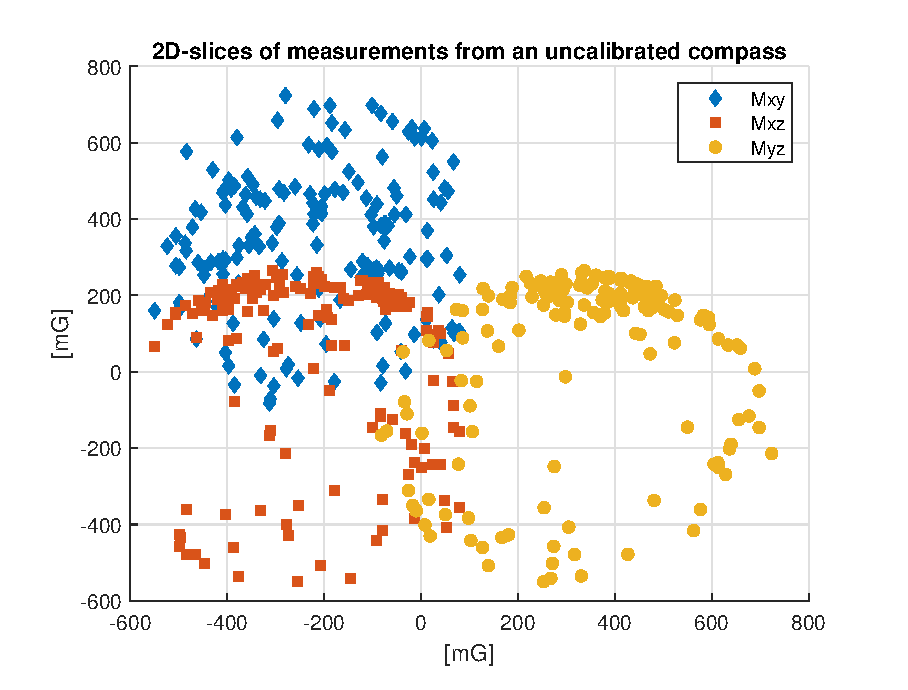
\includegraphics[width=0.96\textwidth]{figures/sensors/board3_uncalibrated_scatterplot.eps}
        \caption{Uncalibrated 2D-slice measurements from the magnetometer on \texttt{arm 3}}
        \label{fig:uncalibcompass}
    \end{minipage}%
    \hspace{.03\textwidth}
    \begin{minipage}[t]{0.48\textwidth}
        \centering
        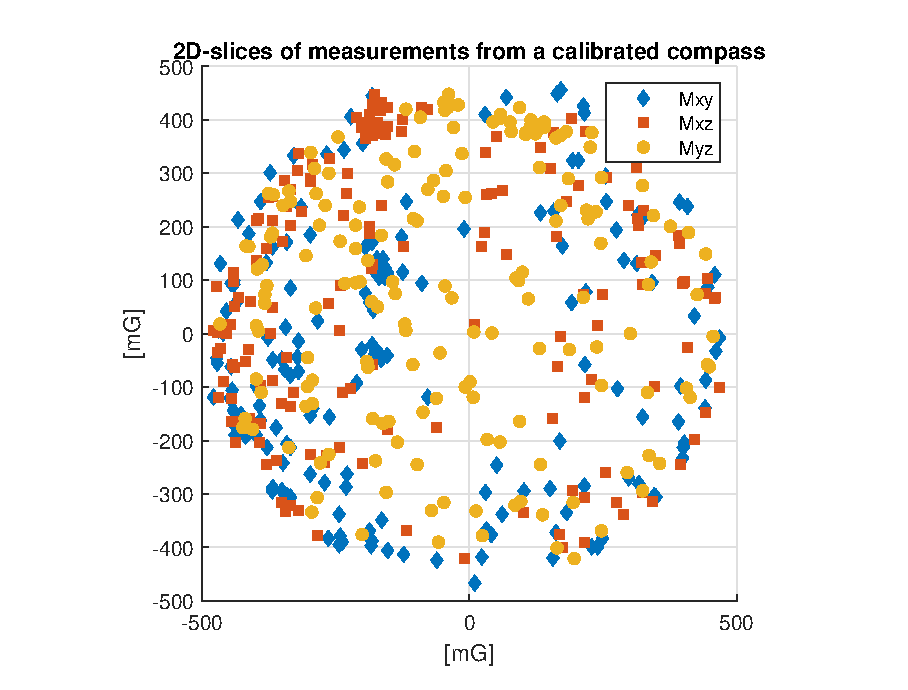
\includegraphics[width=0.96\textwidth]{figures/sensors/board3_calibrated_scatterplot.eps}
        \caption{Calibrated 2D-slice measurements from the magnetometer on \texttt{arm 3}}
        \label{fig:calibcompass}
    \end{minipage}
\end{figure} 

\section{Drone orientation}
The orientation of the drone is found by using measurements from the IMU and a sensor fusion algorithm. When working with orientation in 3 dimensions, Euler angles are typically used, but for this application with a continuous rotation object, quaternions are preferred. Euler angles are three angles used to describe the orientation of a rigid body with regards to a fixed coordinate system. The sequence and axis of which the rotations are made, changes the angles, and thus a convention must exist. In aerospace, the most common one is 'Tait-Bryan' angles. It is from this convention that the names roll, pitch and yaw originate. Euler angles are an easy and intuitive way to describe orientation, but have its disadvantages. Further details of Euler angles will not be discussed, only how they fare compared to quaternions. The difference between quaternions and Euler angles will be analyzed, after a brief introduction of quaternions.\\ 


Quaternions are 4-dimensional vectors, with four real coefficients and three imaginary components, typically denoted with i, j, k, usually on the following form:
\begin{equation*}
    \textbf{q} = [q_0, q_1, q_2, q_3] = a + bi + cj + dk
\end{equation*}
where a, b, c, d are real numbers. It can be seen as a scalar \textit{a}, and a three dimensional vector $bi + cj + dk$ . Like regular complex numbers, they can be written on different forms. Quaternions can be used for many things, but are especially useful for describing orientation of 3D objects. When using quaternions for describing rotations, they must be of unit length. When of unit length, the quaternions describe a 3D space on the surface of a hypersphere. Each point on the hypersphere described by a unit quaternion corresponds to a rotation of a 3D object. 
Additional details about quaternions and how they work will not be discussed further, only how they relate to Euler angles.\\

Quaternions are superior to Euler angles for describing rotating objects, especially ones that laps themselves. This is both due to dealing with edge cases like going from 0 to 360 degrees when completing a full rotation, but they also resolve the problem of singularities. Singularities occur with Euler angles when two angles align. This might happen when the second angle moves in such a way that the first and third angle align, losing one degree of freedom. A third benefit is their improved accuracy when integrating over incremental changes in attitude over time \cite{JamesDiebelQuaternions}. \\
%In the control loops for wing tilt, a quaternion based approach will be used, to maintain the benefits compared to traditional Euler angles.\\
As mentioned, when using quaternions to describe rotations, it is essential to note that they are of unit length. The length of a quaternion is found as in equation \ref{eq:normquaternion}. 

\begin{equation} \label{eq:normquaternion}
    ||q|| = \sqrt{q_0^2 + q_1^2 + q_2^2 + q_3^2}
\end{equation}

When converting from unit quaternions to Euler angles, it is crucial to note the sequence of angles. The microcontroller runs a library written by Kris Winer, that utilizes quaternions, such that a stable orientation can be read from the IMU \cite{kriswinermpu9250}. The library implements two filter fusion algorithms: Madgwick and Mahony filters. For converting between quaternions and Euler angles, the library uses 'Tait-Bryan' notation, which also is known as a 1,2,3 sequence \cite{JamesDiebelQuaternions}.
With this notation, the series of calculations is yaw, then pitch, then roll. If the order of rotation is changed, the result is an entirely different set of angles. 

Eq. \ref{eq:uq2ea1}, \ref{eq:uq2ea2} and \ref{eq:uq2ea3} are the equations used by Kris Winer for converting unit quaternions to Euler angles. 
\begin{align} \label{eq:uq2ea1}
      yaw = \psi &= arctan\left(2\cdot (q_1 q_2 + q_0 q_3), \, q_0^2 + q_1^2 - q_2^2 - q_3^2    \right)\\\label{eq:uq2ea2}
    pitch = \theta &= -arcsin\left(  2\cdot(q_1 q_3 -q_0 q_2)   \right)\\
     roll = \phi &= arctan\left( 2\cdot (q_1 q_2 +q_2 q_3), \, q_0^2 -q_1^2 -q_2^2 +q_3^2 \right)\label{eq:uq2ea3}
\end{align}
As noted in the library, for the IMU's coordinate system, positive z-direction is down towards earth, resulting in a positive sign of the gravitational force. With the local declination of the earth's magnetic field taken into account, yaw is the angle between the sensor's x-axis and the true North. 
Pitch is the angle between the sensor's x-axis and the earth's ground plane, towards the earth is positive. Roll is the angle between the sensor's y-axis and the earth's ground plane, towards the earth is negative \cite{kriswinermpu9250}.

As for the filter fusion algorithm, the microcontroller runs Kris Winer's implementation of a Madgwick filter. This filter combines all data from the IMU (accelerometer, gyroscope, and magnetometer) and calculates the unit quaternions that describe the IMU's absolute orientation. 
A Mahony filter was considered, as well. Kris Winer describes the Mahony filter, as similar to the Madgwick filter, but with proportional and integral filtering on the error \cite{quaternionFilters}. This could potentially result in a filter with less drift of values compared to the Madgwick filter. The drone experienced the best performance with the Madgwick filter. This is also supported by at least one source that compared the two \cite{madgwickvsmahony}. The sensitivity of the gyroscope is set to 2000 DPS, which corresponds to approximately six full rotations per second. 
% link: https://x-io.co.uk/open-source-imu-and-ahrs-algorithms/

\section{Chapter summary}
The IMU was calibrated to fit its measurements more accurately to the drone's position. Euler angles and quaternions were introduced, and their pros and cons discussed. Two filter fusion algorithms were presented, as a way of estimating the drone's orientation. The objectives outlined in section \ref{sensorgoals} have been analyzed and are ready to be tested. The performance will be assessed in section \ref{results:measurementprecision}. 
\chapter{Control loop}\label{controlloopchapter}
In this chapter the simplified physics and SISO linear control theory will be presented. First, the physical link between hover and rotation is developed in section \ref{sec:preliminaryphysics}. Afterwards, constraints of the drone are examined. Finally, how to derive a transfer function for the system, and control it, will be reviewed. Table \ref{tab:constants} shows relevant constants that characterize the system and/or are used for calculations.

\begin{table}[h!]
\centering
\renewcommand{\arraystretch}{1.3}
\begin{tabular}{|l|l|l|}
\hline
Description                & Notation    & Value \\ \hline
Gravitational acceleration & g           & $9.81 \,\frac{\text{m}}{\text{s}^2}$                              \\ \hline
Mass of drone              & $m_{drone}$ & $1.41 \,\text{kg}$  \\ \hline
Air density                & $\rho$      & $1.225 \,\frac{\text{kg}}{\text{m}^3}$                             \\ \hline
Length of arm              & $l_{arm}$   & $0.27\,\text{m}$                              \\ \hline
Length of wing             & $l_{wing}$  & $0.64\,\text{m}$                              \\ \hline
Area of wing               & $A_{wing}$  & $0.121\,\text{m}^2$ (fig. \ref{fig:wing_area_approx})                             \\ \hline
Motor velocity constant    & $K_v$       & $2300$\, $\frac{\text{RPM}}{\text{V}}$       \\ \hline
Motor torque constant      & $K_T$       & $0.0042\, \frac{\text{N}\cdot\text{m}}{\text{A}}$                            \\ \hline
\end{tabular}
\caption{Table of relevant constants}
\label{tab:constants}
\end{table}

\section{Preliminary physics}\label{sec:preliminaryphysics}
For hover conditions, the forces acting on the drone sum to zero. The physical forces acting on each arm are illustrated in fig. \ref{fig:kraftdiagram}.
\begin{figure}[h!]
    \centering
    \includegraphics[width=0.7\textwidth]{figures/control_loops/hover_kraftdiagram.pdf}
    \caption{Diagram of the forces acting on each wing in a hover state}
    \label{fig:kraftdiagram}
\end{figure}
The gravitational forces and lift are calculated for the entire drone (eq. \ref{eq:gravity}), while the horizontal forces of thrust and drag are characterized as internal forces acting on each wing and arm of the drone.  
\begin{equation}
\label{eq:gravity}
    F_t = \frac{1}{3}\cdot m_{drone} \cdot g 
\end{equation}
For hover conditions, the lift must be equal to the gravity acting on the drone, necessitated by Newton's second law of motion. \\
The lift, or upwards thrust, is characterized as (\cite{flight_physics}) the lift induced by a conventional tapered airfoil (eq. \ref{eq:lift}). Eq. \ref{eq:rot2speed} is used when converting from angular velocity to velocity.
\begin{align}
    \label{eq:lift}
    L &= \frac{1}{2}*\rho*v^2*A_{wing}*c_L\\
    v &= \omega * r \label{eq:rot2speed}
\end{align}
$\rho$ is the density of the air.
$A_{wing}$ is the surface area of the wing, which has been approximated as shown in fig. \ref{fig:wing_area_approx}.
\begin{figure}[h!]
    \centering
    \includegraphics[width=0.9\textwidth]{figures/control_loops/wing_area_approx.jpg}
    \caption{Approximation of wing surface area}
    \label{fig:wing_area_approx}
\end{figure}\\ 
Since the wings are rotating around the center, the wings' speed will be proportionately larger further away from the center. The wings' velocity can be modelled as a function of their rotational velocity, $\omega$ (eq. \ref{eq:rotvel}). 
The average rotational velocity is calculated from "copying" the wing into N wings, each with a velocity corresponding to the inner radius plus its iterational value (ie \textit{i}), or number (eq. \ref{eq:omega_approx}). This is done with a simple for-loop that sums all rotational velocities, $\omega$, and divides with the number of wings, N. For increasingly larger N, this number converges to a slightly better approximation than that of a regular mean over the wing's length. $N=10^6$ was found to be an appropriate size. 
\begin{align}\label{eq:rotvel}
    \omega_i &= \frac{\sqrt{\frac{\frac{2}{3}*m_{drone}*g}{\rho*c_L*A_{wing}}}}{r_{inner}+\frac{i*L_{wing}}{N}}\\
    \omega_{avg} &= \frac{\sum_{i=0}^{N} \omega_i}{N+1}
    \label{eq:omega_approx}
\end{align}
The final variable, $c_L$, is set to a constant value for this calculation.
The lift coefficient, $c_L$, is dependent on the angle of attack (AoA) and can be experimentally calculated. The drag coefficient (denoted $c_D$) and lift coefficient, are calculated with NASA's Foil Sim applet for airfoil approximations. The wing's characteristics can be seen in fig. \ref{fig:liftcoefficient} \cite{lift_coefficient}.

The ratio between lift and drag is also calculated with the applet and can be seen in fig. \ref{fig:LDratio}.

\begin{figure}[h!]
    \centering
    \begin{minipage}[t]{0.48\textwidth}
        \centering
        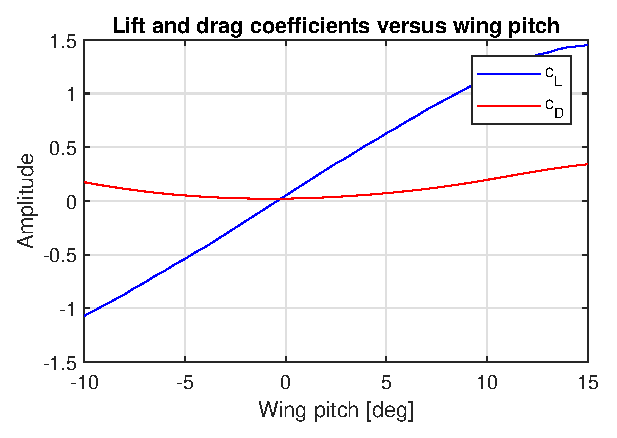
\includegraphics[width=0.96\textwidth]{figures/control_loops/lift_drag_coefficient.eps}
        \caption{The theoretical lift and drag coefficient as a function of the AoA}
        \label{fig:liftcoefficient}
    \end{minipage}%
    \hspace{.03\textwidth}
    \begin{minipage}[t]{0.48\textwidth}
        \centering
        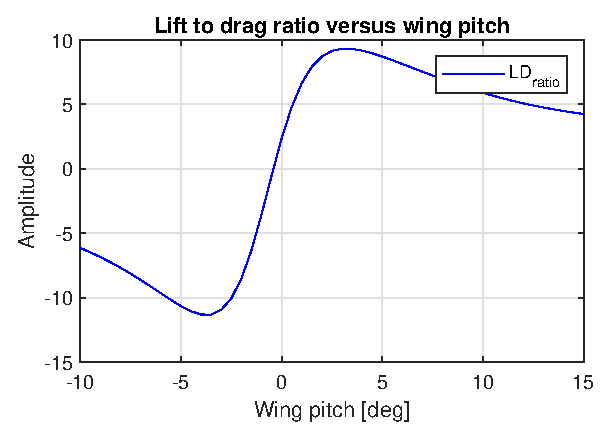
\includegraphics[width=0.96\textwidth]{figures/control_loops/lift_drag_ratio.eps}
        \caption{The theoretical lift-to-drag ratio as a function of AoA}
        \label{fig:LDratio}
    \end{minipage}
\end{figure} 
Although the drone's horizontal axis will be spinning at a constant speed, it is increasingly difficult to calculate and approximate the thrust generated from a propeller motor. Therefore, calculating the motor voltage to lift ratio would require far too many approximations. As such, the results would carry no relevant information to the drone's practical characteristics and, therefore, has not been done. 
Henceforth, the angular velocity will be the measure of the physical model's accuracy.

Varying the lift coefficient, $c_L$, while using the method in eq. \ref{eq:omega_approx}, yields rotational velocities as shown in fig. \ref{fig:liftvariation}

\begin{figure}[h!]
    \centering
    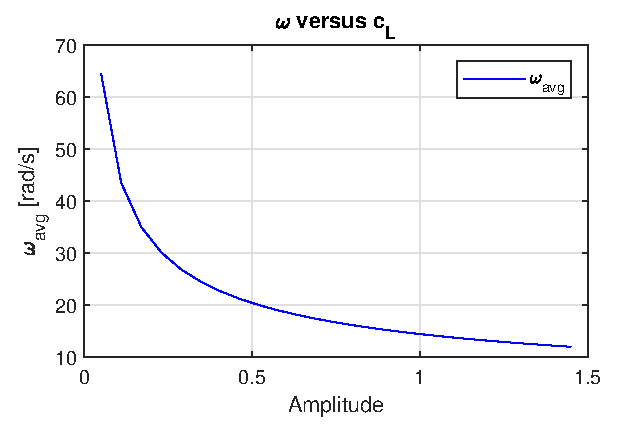
\includegraphics[width=0.5\textwidth]{figures/control_loops/omega_lift_approximation.eps}
    \caption{The average rotational velocity required to hover as a function of the lift coefficient, $c_L$, ($N=10^6$)}
    \label{fig:liftvariation}
\end{figure}

\section{Constraints}
The drone has some physical constraints related to how it was constructed, as it is an atypical drone design. These constraints will have to be considered in the assembly of the control loop.
\begin{itemize}
\label{list:constraints}
    \item The motors are wired in such a way that they are only provided positive voltages. Consequently, they will only be able to spin clockwise (spinning the drone counter-clockwise), thereby creating thrust in their positive z-direction (one-way horizontal rotation).
    \item The wing pitch is very restricted in articulation, as seen in fig. \ref{fig:liftcoefficient}. Any AoA out of this range will most likely cause stalling.
\end{itemize}

\section{System controller}
In this section, design of the system controller will be examined. To be able to control the angular velocity, the drone's physical properties from motor voltage to rotation need to be determined. This means deriving the natural transfer function, which can be found from the step response of the system. 
The finished control system consists of one controller, that will regulate the drone's angular velocity around its z-axis based on a set reference point. \\
The controller will output voltages that adjust the propeller motors to maintain a steady velocity.

\subsection{Natural transfer function of the system}
In this section, it is discussed how a natural transfer function for the system can be derived. The drone will receive a step in voltage, when it's in a steady state rotation, where the output angular velocity will be analyzed both manually and correlated with the assistance of Matlab's Systems Identification Toolbox \cite{SysidToolbox}. This step will be conducted both on- and off-ground.\\

\textbf{Deriving a transfer function:}\\ \label{tf_teori}Manually deriving a transfer function from an open-loop step response can realistically only be done for a very simple system with one or two poles in the same location. For the 2nd order system with coinciding poles, the damping ratio is unity. This is also known as the over-dampened case. Here, the poles are real and negative.
To find this pole, the time constant, $\tau$, must be found. $\tau$ is located as the point in time when the output has reached 63.2\% of its final value. The pole is then found as the negative inverse of $\tau$ \cite{reguleringsbog}. For a 1st order system of the following form, $h(s) = \frac{b}{s+a}$, the static gain is found as $\frac{b}{a}$. From this expression, \textit{b} can be isolated. 

Otherwise, to determine a transfer function for a system, a tool like System Identification Toolbox is useful \cite{SysidToolbox}. It uses a nonlinear least-squares algorithm to fit a user-specified number of poles and zeros to the given data. The data is a step starting from 0, both with input values and output values. It returns a fitted transfer function and a percentage of how good the fit is. 

When analysing the results, a 1st order transfer function will be derived manually once. Thereafter, System Identification Toolbox will be used instead. 

\subsection{Controller type}
As previously mentioned, the drone has physical constraints, therefore the implemented controller will need to have an insignificant overshoot. A differential controller of the right proportions will ensure the right amount of damping and that the overshoot is minimal or non-existent. \\
To ensure minimal steady-state error along with system stability and a fast-enough response, a proportional gain is a natural addition to the differential part. However, the proportional gain is restricted to small values due to the physical constraints of the prop motors' input voltage range. \\
Furthermore, in the process of keeping the controller's response precise and relevant, a simple feed-forward element will be implemented to account for any significant discrepancies. The feed-forward branch works to complement the feedback PD-controller, as it maintains a rather fast overall response of the system. \\
The block diagram is in fig. \ref{fig:controlblock}.

\begin{figure}[h!]
    \centering
    \includegraphics[width=1.0\textwidth]{figures/control_loops/control_block_diagram.png}
    \caption{Block diagram of PD control loop with a feed-forward branch}
    \label{fig:controlblock}
\end{figure}

The values of $K_P$ and $K_D$ will be determined from the system transfer function. The feed-forward gain, $K_f$ will be found by approximating the linear relationship between motor voltage and angular velocity. From this, an expression will be derived. It will act as a system "predictor". \\
For the system, the feed-forward will act as a coarse adjuster, while the PD-controller will act as a fine-tuner.\\
The final closed-loop transfer function becomes (with system named $A(s)$):
\begin{equation}
    G(s) = \frac{\omega_{out}(s)}{\omega_{ref}(s)} = \frac{A(s)*\left(PD(s)+K_f\right)}{1+A(s)*PD(s)}
\end{equation}


\section{Chapter summary}
This chapter introduced the physics of the drone in a hover state. An approximation of the wings' properties was derived, and a controller to regulate the drone's angular velocity was proposed. Additionally its block diagram as well as transfer function were examined. Finally, ways of determining a transfer function from a step response was elaborated upon.\\
The groundwork for a well-functioning control loop has been made. Derivation and implementation of transfer functions and control loop, as well as performance evaluation will be completed in section \ref{results:rotcontroller}.  

\chapter{System modelling}\label{chap:systemmodelling}
For the system modeling, the simplified physics to calculate lift and rotational velocity of the drone from section \ref{sec:preliminaryphysics} will be used. The model is implemented with Simscape Multibody, an add-on of Matlab Simulink.\\

The drone body was developed in Solidworks, seen in fig. \ref{fig:drone3D}. The PCBs, RPi, and battery pack have been assumed as an equal mass distribution on each arm of the drone. As such, they have not been implemented visually in the model.
\begin{figure}[h!]
    \centering
    \includegraphics[width=0.7\textwidth]{figures/system_modelling/drone3d.PNG}
    \caption{3D model of the drone's body excluding wings and propeller motors -- constructed in Solidworks}
    \label{fig:drone3D}
\end{figure}
Subsequently, the motors and wings were added to the model to simulate the physical forces acting on the drone. The physics are also implemented using the equations of chapter \ref{sec:preliminaryphysics}. Although for the sake of computational simplicity, the lift is generated by eq. \ref{eq:model_lift}.\\
\begin{equation}
    \label{eq:model_lift}
    L = \frac{1}{2}*A_{wing}*c_L*\rho*\left(\omega*\left(r_{inner}+\frac{L_{wing}}{2}\right)\right)^2
\end{equation}
The wings' drag and lift coefficient are dynamic and thus implemented with a look-up table.\\

The final model is implemented with many subsystems that model different physical properties. The model consists of subsystems for: 
\begin{itemize}[noitemsep]
    \item Wing physics
    \item Motor physics
    \item Coordinate reference
    \item Controller blocks
    \item Measurement facilitation in all of the above
\end{itemize}

The final visual appearance of the modelled drone is shown in fig. \ref{fig:fullmodeldrone}.
\begin{figure}[h!]
    \centering
    \includegraphics[width=0.5\textwidth]{figures/system_modelling/drone_full_physical_appearance.PNG}
    \caption{The drone model with wings and prop motors}
    \label{fig:fullmodeldrone}
\end{figure}

The top level of the Simulink model can be seen in fig. \ref{fig:toplevelmodel}.

\section{From reality to model and back}
The drag of both motors and wings will be adjusted so that the model fits the real drone's measured data while airborne. \\
The model's natural transfer function will be derived in the same way as with the drone. This is done by stepping the drone at a steady-state. \\

As a result, the model will be used to implement and adjust any proposed rotational controller quickly. Furthermore, it is agile and easy to adjust for changes to the system, or to include new controllers of i.e., height or tilt. The model files are attached to the hand-in.

\section{Chapter summary}
A model of the drone using simplified physics has been implemented using Simscape Multibody in Matlab. The objective outlined in section \ref{modelgoals} has been achieved. Deriving a transfer function and comparing the model with the actual drone will be done in section \ref{sec:modelresponse}. 
\chapter{Results}\label{chap:results}
The goal of this chapter is to test the proposed solutions mentioned in the previous chapters and review their performance. 
\section{Test setups}
Two different test setups are used when assessing the performance of the drone. One setup for testing on the ground, and one setup for simulating in-air behaviour. 

\subsection{Ground}
The ground test rig consists of a rod that the drone can rotate about, to minimize unwanted behavior. The first iteration can be seen in fig. \ref{fig:testsetup_ground}. For the second iteration, a large sheet of wood for the drone to rotate on was added to reduce friction from the surface. The rod material was changed from aluminum to carbon fiber to reduce magnetic disturbances.
\begin{figure}[h]
    \centering
    \includegraphics[width=0.7\textwidth]{figures/results/IMG_0253.JPG}
    \caption{First iteration of the test setup on ground, prior to the second and more stable version of this setup}
    \label{fig:testsetup_ground}
\end{figure}

When estimating the orientation of the drone, a compass rose was put in between the drone and the sheet of wood. North on the compass rose was aligned with true north by use of a compass on a smartphone. 

This setup was used to test measurement precision and derive a transfer function for the system on the ground. 

During the first round of tests, the drone's center module collapsed (see fig. \ref{fig:dronecollapse}). Therefore, a new, more rigid, and sturdy center module was 3D printed.

\begin{figure}[h]
    \centering
    \includegraphics[width=0.7\textwidth]{figures/results/IMG_0274.JPG}
    \caption{Close-up of collapsed center module of the drone after an early test run}
    \label{fig:dronecollapse}
\end{figure}
\FloatBarrier


\subsection{"In-air"}
In this setup (see fig. \ref{fig:testsetup_air}), the drone is suspended from the wooden beam by a thin cord. This cord is so thin that it can easily rotate many times about itself without breaking. Between the cord and the beam, a suitcase-scale is attached. The scale will measure how much lift the drone can generate. The wooden beam is attached to the solid post seen to the left with a rope. 
This setup frees the drone from any friction that was introduced by the wheels. 

This setup was used for wing estimations, getting a transfer function for the system in the air, and testing control loops. 

\begin{figure}[h]
    \centering
    \includegraphics[width=0.7\textwidth]{figures/results/testsetup_air.jpeg}
    \caption{Test setup, air. The drone is hanging from a wooden beam in a cord to simulate in-air behavior}
    \label{fig:testsetup_air}
\end{figure}

\section{Measurement precision}\label{results:measurementprecision}
The precision of the sensor data is crucial for implementing and maintaining reliable controllers on the drone. Thereafter, both the angular velocity and orientation estimations received from the drone are analyzed. 


\subsection{Angular velocity}
The drone's angular velocity sensing is tested by rotating the drone at a constant speed. The rotation is recorded with a video camera and analyzed on a computer. The velocity is tested at PWM of 45\% and 60\% using the ground setup. A comparison of the gathered and recorded data will be made. In this comparison, the measurement of rotational velocity will be converted to rotations per second, because it is challenging to read rotation in radians per second from a video. 

The results of the analysis can be seen in fig. \ref{fig:RPS45PWM} and \ref{fig:RPS60PWM}. 
\begin{figure}[h!]
    \centering
    \begin{minipage}[t]{0.48\textwidth}
        \centering
        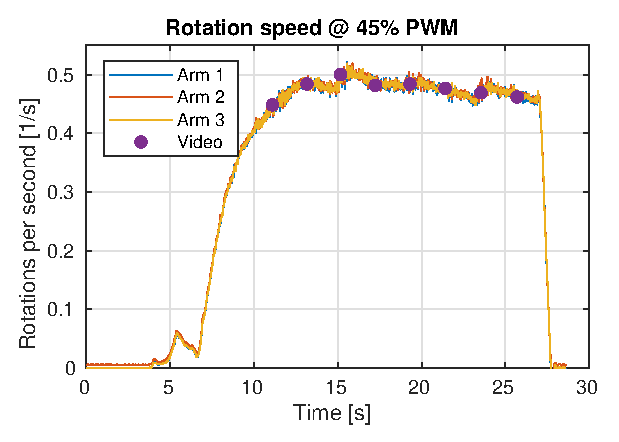
\includegraphics[width=1\textwidth]{figures/results/RPS_45PWM_compared.eps}
    \caption{Rotations per second for PWM at 45\% on ground. Purple dots are from video analysis}
    \label{fig:RPS45PWM}
    \end{minipage}%
    \hspace{.03\textwidth}
    \begin{minipage}[t]{0.48\textwidth}
        \centering
        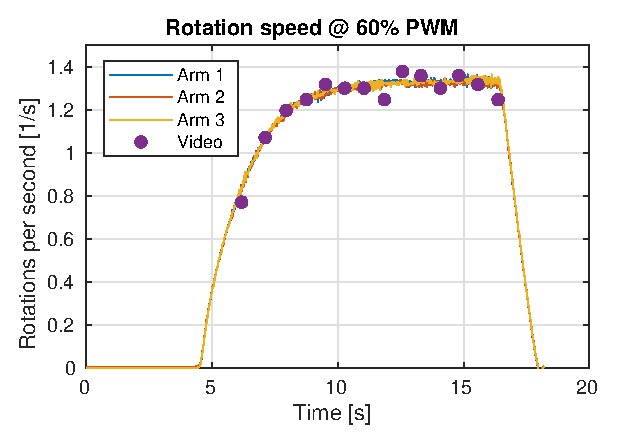
\includegraphics[width=1\textwidth]{figures/results/RPS_60PWM_compared.eps}
    \caption{Rotations per second for PWM at 60\% on ground. Purple dots are from video analysis}
    \label{fig:RPS60PWM}
    \end{minipage}
\end{figure} 
\FloatBarrier
The three lines seen on the figures are each arm's measurement of angular velocity converted to rotations per second. The dots are the rotational speed of the drone derived from the video. Each rotation after the drone started is found and plotted. The start of the recording and start of the drone is lined up as best as possible.


Visually, the distance between points and fits looks very low, especially for PWM at 45\%. The mean square error of the points from the video compared to the sensor data is found to be $MSE_{PWM=45\%} = 6.8220\cdot 10^{-5}$ and $MSE_{PWM=60\%} = 1.8*10^{-3}$. From this it can be concluded, that the measurements of rotational velocity are precise and work as expected.






\subsection{Orientation estimation}
The orientation of the drone is described by roll, pitch, and yaw.  The magnetometer on the drone has been corrected for the local declination of the magnetic field. With the correction, yaw measures the angle from the IMU's x-axis to the true north. 
The ground test-setup was used to examine the drone's ability to estimate its orientation. 
While the drone was rotating, it was recorded from an angle directly above it. This was done for PWM at 40\% and 50\%. 

Continuous measurement of yaw with data from all arms can be seen in fig. \ref{fig:rpm40woodallarms}. 


\begin{figure}[h]
    \centering
    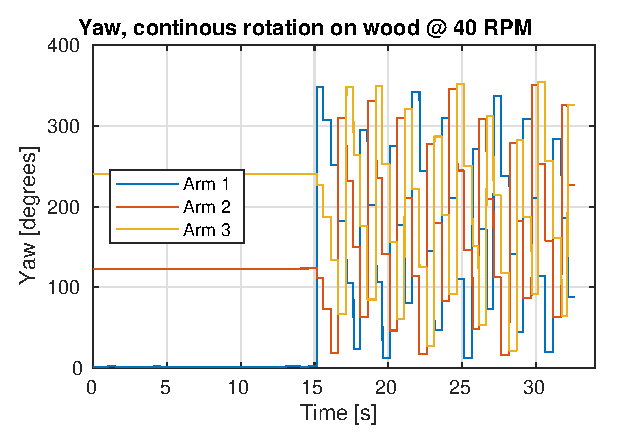
\includegraphics{figures/results/Yaw_rpm40_wood_allarms.eps}
    \caption{Yaw measurements, PWM at 40\% on ground test setup}
    \label{fig:rpm40woodallarms}
\end{figure}
As can be seen, there are about 110 degrees between all arms most of the time. 
The angle doesn't always go all the way to 0 or to 360, but this is also visually exaggerated due to the cyclic nature of angles. Errors related to this will be discussed in section \ref{error_measurementprecision}.


In the analysis of the videos, it was noted each time \texttt{arm 1} had rotated 90 degrees. These points are plotted against \texttt{arm 1's} measurement of the yaw angle. This was done both for RPM at 40\% and 50\% (see fig \ref{fig:rpm40woodvid} and \ref{fig:rpm50woodvid}). 
\begin{figure}[h!]
    \centering
    \begin{minipage}[t]{0.48\textwidth}
        \centering
        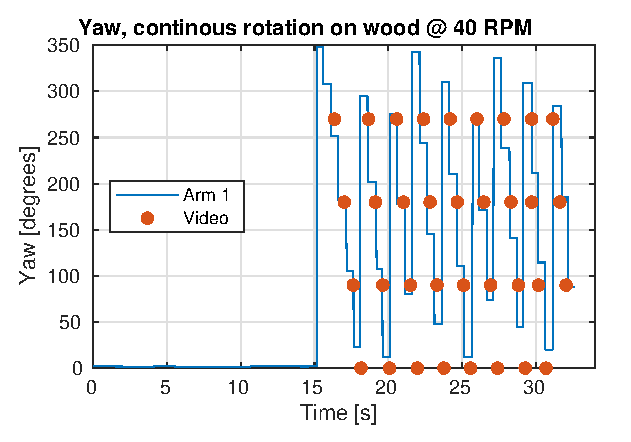
\includegraphics[width=1\textwidth]{figures/results/Yaw_rpm40_wood.eps}
        \caption{Yaw measuremnets, PWM at 40\% on ground test setup, arm 1 and video}
    \label{fig:rpm40woodvid}
    \end{minipage}%
    \hspace{.03\textwidth}
    \begin{minipage}[t]{0.48\textwidth}
        \centering
        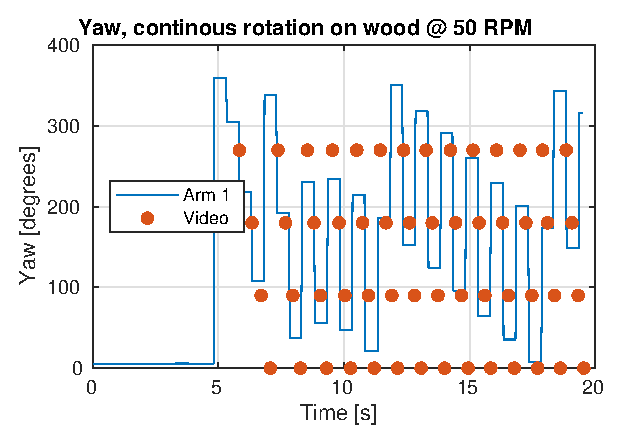
\includegraphics[width=1\textwidth]{figures/results/Yaw_rpm50_wood.eps}
        \caption{Yaw measurements, PWM at 50\% on ground test setup, arm 1 and video}
        \label{fig:rpm50woodvid}
    \end{minipage}
\end{figure} 
Angles of either 0 or 360 degrees from the video analysis, are always plotted as 0 degrees for clarity.
At a PWM of 40 \%, the measured data agree quite well with the video analysis. At higher levels of PWM, the plot starts to lack some data points in the rotation. 

Locating north within $\pm 1$ degrees was never the target goal. A well-calibrated IMU with a Madgwick filter can have a precision of $\pm 4$ degrees \cite{FilterFusionPrecision}. This test shows that it is possible to measure with an accuracy of $\pm 20$ degrees when rotating continuously.  

For the time being, it is somewhat unreliable for higher speeds, but it would be easy to improve (see chapter \ref{sec:communicationimprove}).
Sources of errors and other limitations are discussed in section \ref{error_measurementprecision}.



\subsection{Sources of error} \label{error_measurementprecision}
The general increase in error between video and measured data can be attributed to several things. 
Firstly, due to not having an infinitely high sampling rate on the microcontrollers and its sensors, the error in measurements will naturally increase as the rotational speed increases. 
The sampling rate of the IMU is 100 Hz for the magnetometer, 200 Hz for the gyroscope, and about 1 kHz for the accelerometer. As mentioned previously, the IMU is configured for interrupt-based communication. This limits the update frequency to the lowest common denominator and therefore is 100 Hz. 

Secondly, the video recording was limited to 30 fps. As the picture becomes increasingly blurry, the observer's inability to distinguish angles expectedly grows. The error between the points from the video and the measurements will also increase with velocity. 

Finally, the plots may also make the data look worse than it is. Given that the update frequency only is 30 Hz between RPi and microcontroller, significant data is lost. About 2/3 of all data points are never seen on the RPi, which might explain the lack of "complete rotations" seen in fig. \ref{fig:rpm50woodvid}. At times, the data jumps from 200-300 degrees down to a value slightly above 0 degrees. These jumps are  likely caused by a lack of data on the RPi, rather than lack of data on the microcontroller.

A test of yaw drift can be seen in appendix \ref{fig:yawdrifttest}. It shows no noteworthy drift. 


\section{Wing estimations} \label{chap:wing_est}
The wings' properties were measured with the "in-air" setup. The motors had a constant input voltage, $V_{in} = 3.57 V$ corresponding to a PWM of 30\%. Afterwards, the lift and angular velocity for a varying wing pitch was measured to estimate both the lift and drag coefficients.\\
The lift was measured as a mass with the suitcase-scale on the end of the string carrying the drone. The final lift and angular velocity versus wing pitch can be seen in fig. \ref{fig:lift_omega_measured}.

\begin{figure}[h]
    \centering
    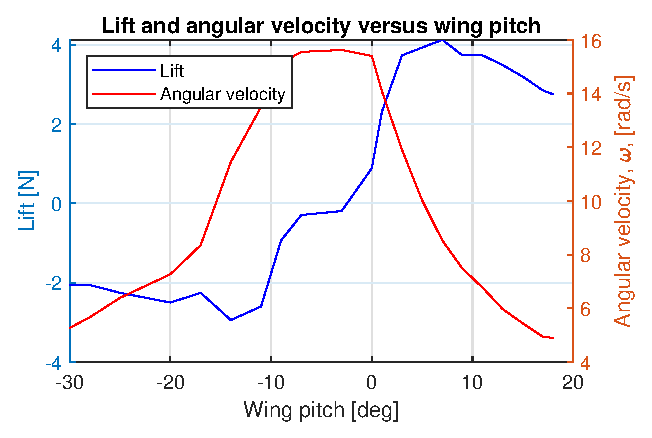
\includegraphics{figures/results/lift_rotation_measured.eps}
    \caption{Lift and angular velocity measured for different wing pitches}
    \label{fig:lift_omega_measured}
\end{figure}

The lift coefficient was estimated from the approach in eq. \ref{eq:cLestimation}. The approach is similar to the one used to calculate the required rotation in eq. \ref{eq:omega_approx}. N is the amount of iterations (here $N=10.000$) and $\Delta R = L_{wing}/N$.
\begin{equation}
\label{eq:cLestimation}
    c_L(\theta) = \frac{1}{3} * \frac{L_{meas}(\theta)*N}{\rho*A_{wing}*\omega^2*\sum_{i=1}^{N} (r_{inner}+ i*\Delta R)^2}
\end{equation}
The comparison of the estimated and measured lift can be seen in fig. \ref{fig:lift_measured}.\\

The drag coefficient at a wing pitch of 0 degrees was adjusted in the Matlab-model until simulations showed similar physical properties to the ones of the drone. This was achieved at a drag coefficient of, $c_{Dbase} = 0.176$ and angular velocity of $\omega_{base} = 15.4 [rad/s]$.\\ 
The subsequent drag coefficients were estimated with eq. \ref{eq:drag_estimation}, since the output power of the motors were the same throughout the test.
\begin{equation}
\label{eq:drag_estimation}
    c_D(\theta) = \left(\frac{\omega_{base}}{\omega_{\theta}}\right)^2* c_{dBase}
\end{equation}
The resulting drag coefficients can be seen compared to the Foil Sim Applet's estimation in fig. \ref{fig:drag_measured}. Furthermore, measured lift coefficients compared to Foil Sim Applet's estimation can be seen in fig \ref{fig:lift_measured}.\\
Both the drag and lift coefficients measured deviate significantly from the ones obtained from the applet. This can be partially explained by the imprecise scale (meant for weighing suitcases) and the fact that the drone does oscillate slightly away from directly underneath the string. These results are prone to many errors caused by a series of underlying approximations and assumptions. The complexity of aerodynamics shall not be underestimated; however, these results work decently for testing purposes.

\begin{figure}[h!]
    \centering
    \begin{minipage}[t]{0.48\textwidth}
        \centering
        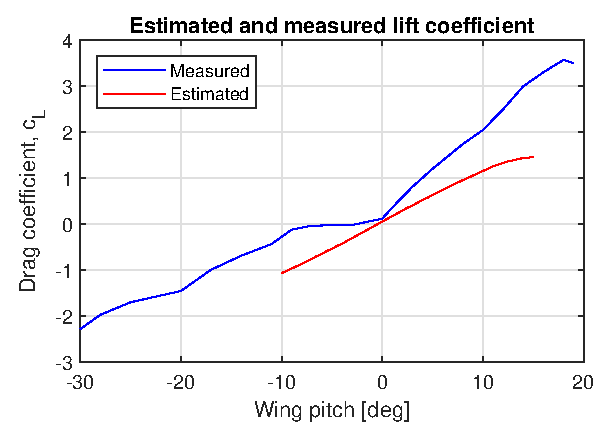
\includegraphics[width=1\textwidth]{figures/results/lift_measured.eps}
    \caption{Lift coefficient measured with the test rig compared to the estimated lift coefficient from the Foil Sim Applet}
    \label{fig:lift_measured}
        
    \end{minipage}%
    \hspace{.03\textwidth}
    \begin{minipage}[t]{0.48\textwidth}
        \centering
        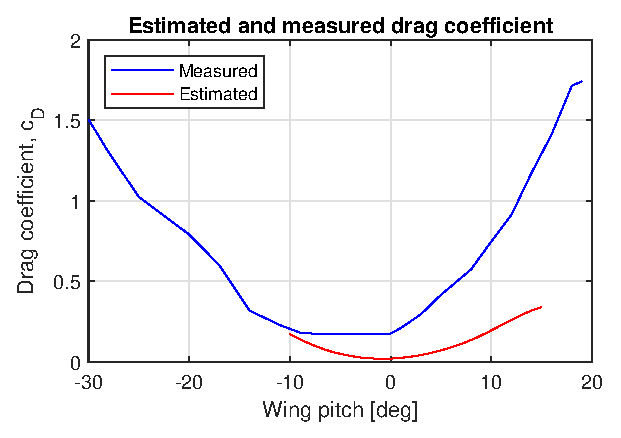
\includegraphics[width=1\textwidth]{figures/results/drag_measured.eps}
    \caption{Drag coefficient measure estimation with the test rig compared to the coefficients from the Foil Sim Applet}
    \label{fig:drag_measured}
    \end{minipage}
\end{figure} 
Fig. \ref{fig:LDratio_measured} is a plot of the lift-to-drag ratio measurement and Foil Sim estimation.
\begin{figure}[h]
    \centering
    \includegraphics{figures/results/LDratio_measured.eps}
    \caption{Lift-to-drag ratio as measured and estimated with the Foil Sim Applet}
    \label{fig:LDratio_measured}
\end{figure}
\newpage

\section{Rotation controller and system response}\label{results:rotcontroller}
Transfer functions will be derived for the system in three different states and one for the model. First state is a grounded system. Second state is in the air with minimal drag. Third state is in the air with some drag. The functions will be analyzed and compared to each other, to examine the difference between states as well as model compared to the real world. 
Eventually the final controller will be derived and implemented. 


\subsection{Deriving transfer functions}
To derive a transfer function, the theory in section \ref{tf_teori} is used. The system received a step of PWM from 35\% to 39\%, and is analysed both on the ground and in the air. This value interval might seem arbitrary, but was chosen, as it is high enough to let the drone rotate both on the ground and in the air, yet low enough so the drone is easily observable. Furthermore, in the air, it is stepped both with minimal drag and some drag. This was chosen to investigate if there was any notable difference between the system responses in the three cases. 
% When using System Identification Toolbox, a guess of a system with 1 pole and 2 poles are made. This is due to having a low sampling frequency, so time constants from the motors and other really fast components are not visible. One constant is expected from the inertia of the drone due to its size, and one for 

\subsubsection{Grounded system}
The step from PWM of 35 \% to 39\% is made using the ground test-setup and can be seen in fig. \ref{fig:stepwood}.
\begin{figure}[h!]
    \centering
    \begin{minipage}[t]{0.48\textwidth}
        \centering
        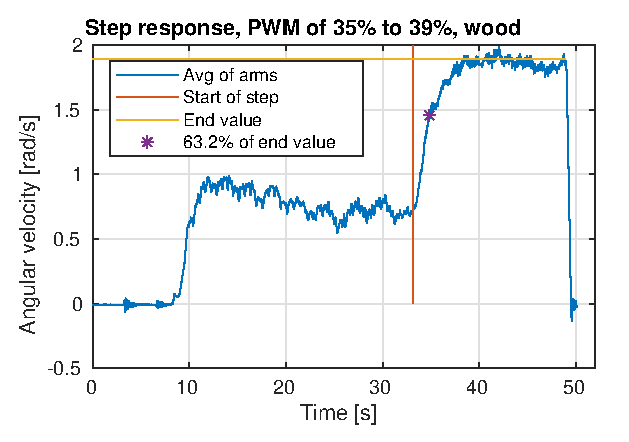
\includegraphics[width=1\textwidth]{figures/results/stepwood.eps}
        \caption{Step on wooden surface using the ground test-setup}
        \label{fig:stepwood}
    \end{minipage}%
    \hspace{.03\textwidth}
    \begin{minipage}[t]{0.48\textwidth}
        \centering
        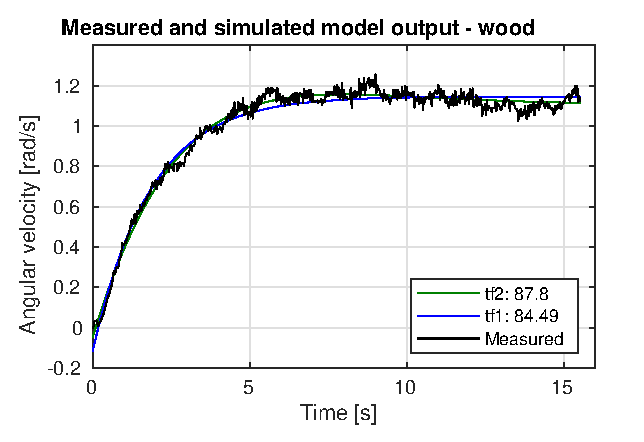
\includegraphics[width=1\textwidth]{figures/results/stepwood_sysid.eps}
        \caption{Plot from System Identification Toolbox. $Tf_1$ is 1 pole, $Tf_2$ is two poles. The data was offset to start in 0}
        \label{fig:stepwoodsysid}
    \end{minipage}
\end{figure} 
This looks quite similar to a 1st or 2nd order system. One might expect a system with more poles, but with the low sampling frequency smaller time constants (e.g. electrical) cannot be measured. \\
Assuming a 1st order system and analysing the step, the time constant is found as $\tau_1 = 1.6404$. The pole is $p_1 = -0.6096$. \textit{b} can then be calculated:

\begin{equation}
    b = \frac{y_{final} - y_{init}}{x_{final}}* a =  \frac{1.89-0.71}{4.5} \cdot 0.6096 = 0.1603
\end{equation}

The manually derived transfer function becomes:
\begin{equation}\label{eq:woodsysman}
    tf_{manual} = \frac{0.1603}{s+0.6096}
\end{equation}

Analysing the step with System Identification Toolbox, the following step and transfer functions are derived, see fig. \ref{fig:stepwoodsysid} as well as eq. \ref{eq:woodsysid1} and \ref{eq:woodsysid2}. 


\begin{equation}\label{eq:woodsysid1}
    tf_1 = \frac{0.1387}{s+0.5383}
\end{equation}
\begin{equation}\label{eq:woodsysid2}
    tf_2 = \frac{0.03641}{s^2 + 0.6571 s + 0.1462}
\end{equation}
The transfer function found manually in eq. \ref{eq:woodsysman} and the two found with System Identification Toolbox, are very similar. The two 1st order systems have poles in approximately the same places and almost the same gain. 
The 2nd order system has a complex pole pair located at $-3.29 \pm 0.196 I$. The complex poles are presumably caused by either flex in the wheel mounting, or due to the vibration introduced from the wooden surface. 






\subsubsection{Airborne system with minimal drag}\label{sec:airminimal}
The step of the system was made with the air test-setup, see fig. \ref{fig:steprope}.
\begin{figure}[h!]
    \centering
    \begin{minipage}[t]{0.48\textwidth}
        \centering
        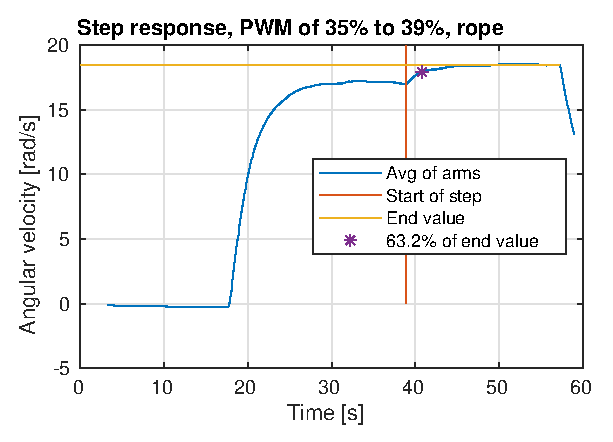
\includegraphics[width=1\textwidth]{figures/results/steprope.eps}
        \caption{Step using air test-setup}
        \label{fig:steprope}
    \end{minipage}%
    \hspace{.03\textwidth}
    \begin{minipage}[t]{0.48\textwidth}
        \centering
        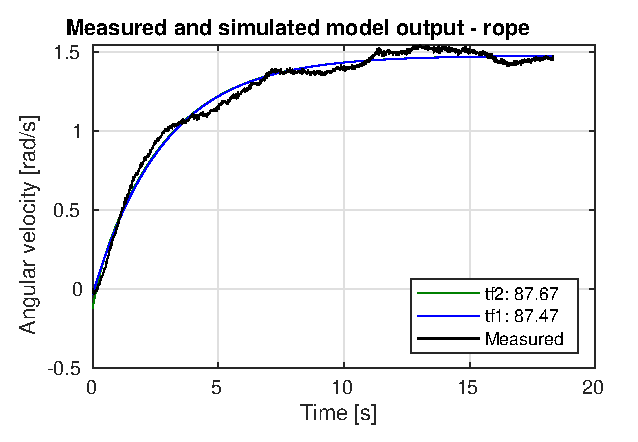
\includegraphics[width=1\textwidth]{figures/results/steprope_sysid.eps}
        \caption{Plot from System Identification Toolbox, $Tf_1$ is 1 pole, $Tf_2$ is 2 poles. The data was offset to start in 0}
        \label{fig:stepropesysid}
    \end{minipage}
\end{figure} 

Analyzing the step with System Identification Toolbox, the fits can be seen in fig. \ref{fig:stepropesysid}, and transfer functions in eq. \ref{eq:airsysid1} and \ref{eq:airsysid2}.

\begin{equation}\label{eq:airsysid1}
    Tf_1 = \frac{0.1132}{s+0.3523}
\end{equation}
\begin{equation}\label{eq:airsysid2}
    Tf_2 = \frac{0.4608}{s^2 + 4.439s+1.434}
\end{equation}
The first pole for the 1st order and 2nd order system is practically identical at respectively $-0.3523$ and $-0.3507$. Due to its very low frequency, this pole probably correlates to the inertia of the drone. \\
The second pole for the 2nd order system is at $-4.088$, and corresponds to a very small time constant. The second, less dominant, pole might possibly be the pole associated with the mechanical time constant of the motors \cite{motordata} (see also section \ref{sec:modelresponse}) .

\subsubsection{Airborne system with more drag}
The step was made using the air test-setup, but this time with a 5 degrees tilt of the wings (positive angles creates lift). The step response can be seen fig. \ref{fig:steprope65}.

\begin{figure}[h!]
    \centering
    \begin{minipage}[t]{0.48\textwidth}
        \centering
        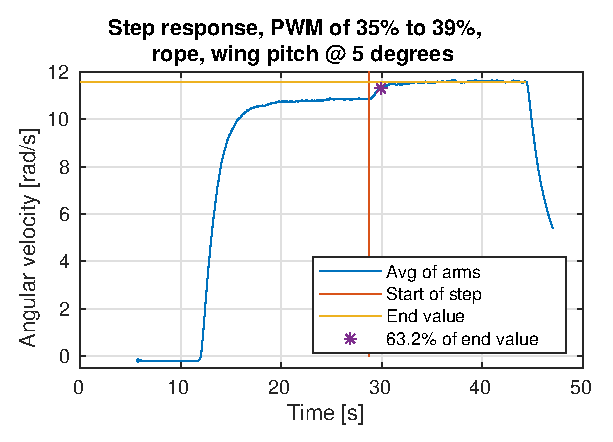
\includegraphics[width=1\textwidth]{figures/results/steprope65degrees.eps}
        \caption{Step using air test-setup with a pitch angle of $\sim$5 degrees}
        \label{fig:steprope65}
    \end{minipage}%
    \hspace{.03\textwidth}
    \begin{minipage}[t]{0.48\textwidth}
        \centering
        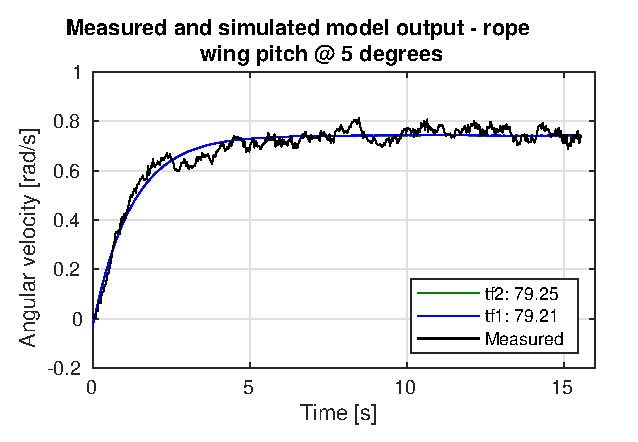
\includegraphics[width=1\textwidth]{figures/results/steprope65degrees_sysid.eps}
        \caption{Plot from System Identification Toolbox, $Tf_1$ is 1 pole, $Tf_2$ is 2 poles. The data was offset to start in 0. Pitch angle was $\sim$5 degrees}
        \label{fig:steprope65sysid}
    \end{minipage}
\end{figure} 

With System Identification Toolbox, the following fits and transfer functions are found, see fig. \ref{fig:steprope65sysid} as well as eq. \ref{eq:air65sysid1} and \ref{eq:air65sysid2}. 


\begin{equation}\label{eq:air65sysid1}
    Tf_1 = \frac{0.1311}{s+0.8044}
\end{equation}
\begin{equation}\label{eq:air65sysid2}
    Tf_2 = \frac{3.862}{s^2 + 29.91s + 23.7}
\end{equation}
The 2nd order system's poles are real and located at $p_1=-0.815$ and $p_2=-29.095$. The first pole from the 2nd order system is very close to the pole from the 1st order system. This second pole is much smaller than the second pole for the case with minimal drag. This clearly outlines some nonlinear component in the system and may very well be caused by the drag. 


\subsubsection{Comparison of systems}
The systems on wheels and in the air are very similar in terms of time constants, but the resistance from rolling associated with the wheels create a large offset. With a PWM of 35\%, the angular velocity in the air is about 16 rad/s, but on the ground, it is approximately 0.8 rad/s. This is a massive loss in rotational energy. Furthermore, the absolute increase in amplitude for the steps on the ground and in the air is about the same, which means the rolling resistance does not increase appreciably with angular velocity. \\ 
The dominating time constant for the case with some drag is faster than the one with minimal drag, but the system also reaches a far lower amplitude. The minimal drag case's relative increase in amplitude is 1.5 but is only 0.75 for the case with some drag. Due to non-linear components, there is a notable difference between the two step-responses, both in terms of steady-state error and pole placement. This can be solved with gain scheduling, though this concept will not be explored further in this thesis. 


\subsection{Modelled system's response}\label{sec:modelresponse}
The model transfer function was derived in a similar fashion to the method above. At a steady state rotation the input voltage of $V_{in} = 0.35*11.9V = 4.17 \,V$ was stepped to $V_{in} = 0.39*11.9V = 4.641\,$. The model's step response was analyzed with the help of the Tfest-function in the System Identification's Toolbox (fig. \ref{fig:bode_tfest}). The steady state gain was measured to 0.9 for the Simulink model.
\begin{figure}[h]
    \centering
    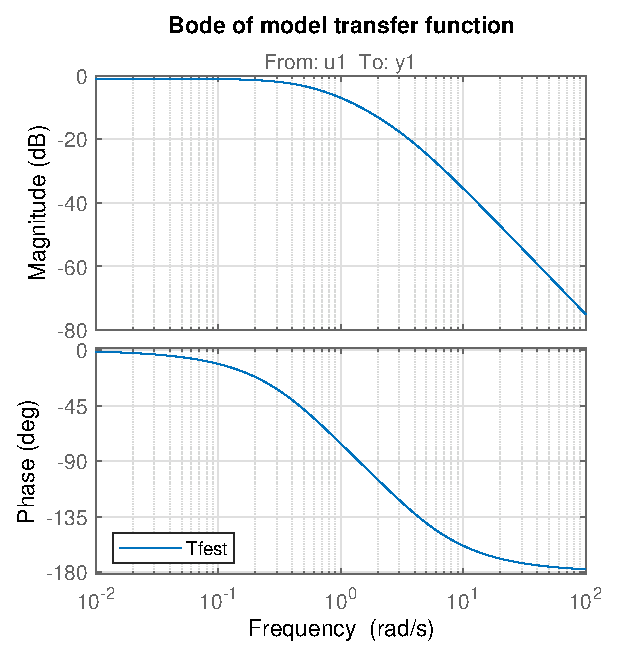
\includegraphics{figures/results/bode_tfest.eps}
    \caption{Bode plot of model's transfer function; voltage to angular velocity}
    \label{fig:bode_tfest}
\end{figure}
The system approximated with Tfest is a 2nd order continuous system, with a fit of 99.4\%. The transfer function for this system is: 
\begin{equation}
    M(s) = \frac{1.77}{s^2+3.82*s+1.96}   
\end{equation}
The poles for this transfer function are $p_1 = -0.61$ and $p_2 = -3.21$. \\
Similarly, by measuring the time constants "by hand" for the drone's angular velocity, $\omega$ and the motors' RPM in the model, the poles become: $p_{\tau \omega} = -0.535$ and $p_{\tau RPM} = -6.87$.  \\
By comparing these two sets of poles, with the transfer function derived in section \ref{sec:airminimal}, it's seen that the modelled system is indeed a good approximation of the real drone. Each pole is roughly within a factor of two of its equivalent pole. Furthermore, it supports the theory that the two lowest frequency poles of the system are associated with the inertia of the system and the mechanical pole in the prop motor.


\subsection{Final controller and implementation}
\subsubsection{Feed-forward gain estimation}
The feed-forward branch was determined by inputting different voltages and recording the drone's steady-state angular velocity. The fit and plot of these data can be seen in fig. \ref{fig:kfestimation}.
\begin{figure}[h!]
    \centering
    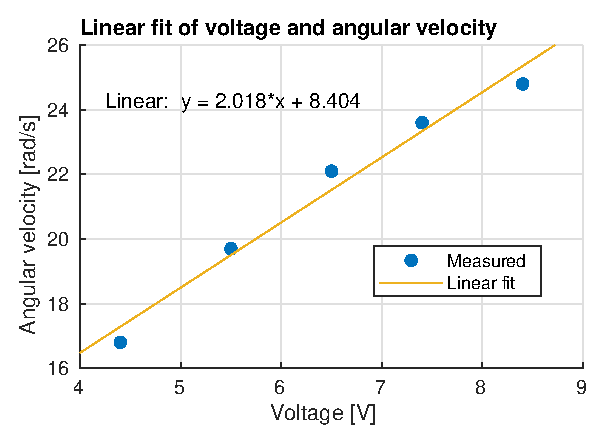
\includegraphics{figures/results/feedforwardfit.eps}
    \caption{Linear fit of angular velocity versus input voltage}
    \label{fig:kfestimation}
\end{figure}
The angular velocity versus input voltage can be approximated as a linear relationship. The gain from the reference $\omega$ to the summation node (see also fig. \ref{fig:controlblock}) before the system becomes:
\begin{equation}
    V = -4.16 + 0.50*\omega_{ref}
\end{equation}
The constant offset is because the motor will not turn on below an input PWM of 13\%.\\

\subsubsection{Proportional and differential gain}
Since the rough input voltage to the system is taken care of by the feed-forward branch, the $K_p$ does not need to be very large. The $K_p$ was found to generate stable results on the model within the ranges of $K_p = [0.7;1.5]$.\\
Equally, the differential gain, $K_d$, needed to be large enough to dampen any unnecessarily large accelerations, but not so large that the response time was too long. For the implementation, the derivative gain was finalized at $K_d = 0.9$. This dampens the oscillations sufficiently.\\
The final implemented controller (including the feed-forward branch) is as seen in eq. \ref{eq:finalcontroller}; $e(t)$ is the time dependent error.
\begin{equation}
    \label{eq:finalcontroller}
    V(t) = 1.3 + 0.9*\frac{de(t)}{dt}+(\omega_{ref}*0.50-4.16)
\end{equation}
The complete system is stable with an infinite phase margin. However, there is a steady-state error of -2.6 dB; see fig. \ref{fig:systemcontrollerbode}. The derived system with the pitched wing is stable with this controller but will experience a larger steady-state error (fig. \ref{fig:systempitchcontrollerbode}). This is because of the generally non-linear behavior of the velocity. The consequence will be, that the controller will not be a one-size-fits-all solution, but rather a compromise of being stable and precise around the operating point of $\theta_{wing} = 0 \,deg$. \\

\subsubsection{Step response with controller}
The drone was tested with the controller using the air setup. It started from an initial velocity of 0 and a reference point of $\omega_{ref} = 15 \, \text{rad/}$. When the drone had reached steady state, its reference point was changed to $\omega_{ref} = 20 \, \text{rad/s}$. The sensor measurements of the step can be seen in fig. \ref{fig:stepwithcontroller}.
\begin{figure}[h]
    \centering
    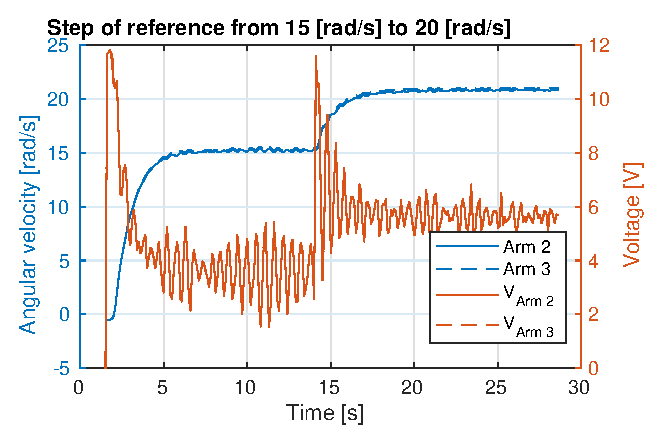
\includegraphics{figures/results/stepwithcontroller.eps}
    \caption{Closed-loop step with controller. From $\omega_{ref} = 15\, \text{rad/s}$ to $\omega_{ref} = 20\, \text{rad/s}$}
    \label{fig:stepwithcontroller}
\end{figure}
For the initial reference point the drone settles at an angular velocity of $\omega_{out} = 15.27 \,\text{rad/s}$.

\begin{table}[h]
\centering
\resizebox{0.5\textwidth}{!}{%
\begin{tabular}{|l|l|}
\hline
Time domain specification & Value \\ \hline
Rise time                 & 2.4 [s] \\ \hline
Settling time             & 9.3 [s] \\ \hline
Peak time                 & 12.1 [s] \\ \hline
Overshoot                 & 4.95 \%     \\ \hline
Steady state error        & $0.92\, [\text{rad}/\text{s}]$ \\ \hline
\end{tabular}%
}
\caption{Time domain specifications for system with controller and feed-forward}
\label{tab:timedomainspecs_step}
\end{table}
For both reference points, the controlled system experiences a steady-state error as one might expect from inspecting the closed-loop frequency response. However, this steady-state error is much smaller than what the closed-loop frequency response indicates.\\
This could be the result of the somewhat low sensor sampling rate of about $f_{s} = 100 \,\text{Hz}$. Some poles related to the constants of the motor are likely to be at much higher frequencies.\\
Furthermore, this steady-state error is a necessary compromise for the system. The proportional gain is limited to small values because the motor voltage is confined to values between 0 and the battery voltage. Thus, this rather small steady-state error is a beneficiary compromise of the stable system. \\
In table \ref{tab:timedomainspecs_step}, the step time domain specifications of the system with controller and feed-forward are listed. The final controlled system is considerably fast with a 2.4s rise time; however, this does introduce some overshoot.\\

Additionally, one of the sensors stopped working for the drone's final testing with the controller, leading to less accurate measurements, which does play a role in the error that the controller uses.



\section{Flying the drone}\label{chap:flydrone}
Finally, the drone is not complete without a proper test flight. The test flight was done while attached to the "in-air" setup. The flight procedure was done without the rotational controller. \\
The procedure for "flying" was:
\begin{enumerate}
    \item Accelerate drone to an obtainable speed at 80\% of the maximal voltage with 0 degree wing pitch
    \item Set the wing pitch to roughly 10 degrees upwards.
\end{enumerate}
\begin{figure}[h]
    \centering
    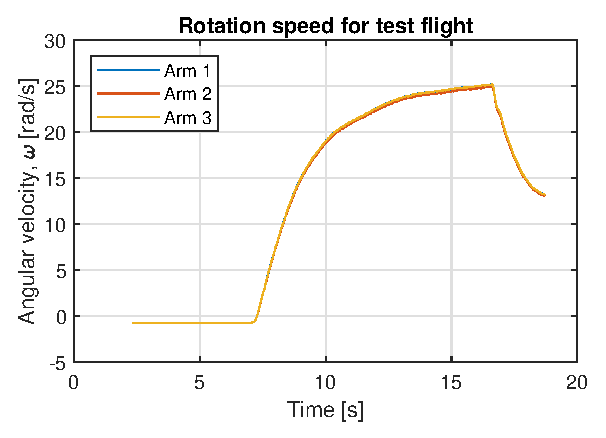
\includegraphics{figures/results/flight_rotational_velocity.eps}
    \caption{Rotational velocity of the drone for flight tests. At $\sim$16.5 seconds, the pitch angle was changed to generate lift}
    \label{fig:rotationflight}
\end{figure}
This procedure did not result in continuous flight but did create a burst of enough lift such that the drone changed its z-position by around $0.5$m above its initial position. Afterwards, it slowly soared down to the original height as all its built-up kinetic energy had been transferred into mechanical lift and drag.\\
Since the motors were only throttled to 80\% of their maximum, they could indeed have been able to sustain a hover condition. However, at very high speeds, the drone loses stability about its horizontal axis and starts swinging heavily from side to side.\\
The rotational velocity seen in fig. \ref{fig:rotationflight} is well above the required rotation for hover with a wing pitch of 10 degrees (fig. \ref{fig:lift_measured}).
A link to a video of the "flight" can be found in appendix \ref{link:droneflight}. 



\section{Power use} \label{sec:poweruse}
With regards to power usage, there are especially two things to be consider when estimating usage. First the prop motors draw a rather large current when running, so any loss within the wires and PCB can be neglected. Secondly, the input current to each PCB can be assumed equal to the input current to the motors. The voltage-power relationship can be seen in fig. \ref{fig:power} (with a wing pitch of $\theta_{wing} = 0 \,deg$). Comparing this angular velocity with the ones calculated in fig. \ref{fig:liftvariation} and the measured lift in fig. \ref{fig:lift_omega_measured}, it is seen that a slight pitch of the wing would indeed slow the drone's rotation, but create the lift necessary to hover. This means that this power output is a decent estimate of the one required in a hover state.\\
\begin{figure}[h!]
    \centering
    \includegraphics{figures/results/power_voltage.eps}
    \caption{Input power of all prop motors versus voltage; includes recorded angular velocity}
    \label{fig:power}
\end{figure}
The power draw is quite low compared to drones like the one mentioned in section \ref{sec:stateoftheart}, but the battery in use is also small. This means, that with the current setup the flight time will not be very long. How to increase the duration will be discussed in section \ref{sec:futureworkphysicalchanges}. 




\section{Chapter summary}
The sensor measurements were tested and found to be successful. Additionally the sensor fusion algorithm was tested. It was seen that the internal sampling rate of the compass in the IMU had a restricting effect on the algorithm's accuracy. The wing approximation was tested with the real drone's behavior at different AoA. The drone's natural transfer function was also derived both on and off ground for further analysis. Furthermore the model's transfer function was derived. The drone's controller was analysed and implemented with success. It was also shown that the drone is able to fly under the right conditions. All objectives outlined in section \ref{sec:objectives} and \ref{analysisofgoals} were achieved. 
\chapter{Future Work}\label{chap:futurework}
Further improvements and future work consist of (but are not limited to):
\begin{itemize}
    \item Physical changes in both wheels and wing types
    \item Increasing RPi sample rate by improving communication
    \item Tilt controller, for a more stable flight
    \item Rotational based height regulator. This would require new height measuring devices e.g., sonic sensor et al.
    \item Software fail-safes to increase robustness and safety of the drone
    \item Exploring other purposes for this drone-type
\end{itemize}

\section{Physical changes}\label{sec:futureworkphysicalchanges}
The most significant drawbacks of the current state of the drone have proven to be the wings and the wheels.\\
As seen from the final flight tests, the drone does not have the necessary power to lift and maintain a hover condition for itself. This can be fixed either with more powerful thrust or larger wings with more lift potential. The former solution bears diminishing returns and has in previous configurations been shown to create unnecessary instability with e.g., larger propellers. The latter solution, however, can prove to be a turning-point as the mass of each wing compared to their lifting capabilities is minuscule. On the contrary, the new wings would probably require a more rigid frame or redesigning the drone structure altogether.\\
The wheels have also shown that they currently introduce a large damping offset when the drone is grounded. This issue will play a rather vital role if the drone was to take off directly from the ground.\\
As seen in section \ref{sec:poweruse} the energy usage of the drone is little (compared to the drones mentioned in section \ref{sec:stateoftheart}), but so is the flight time. 
There are numerous reasons for this low flight time and why it easily can be improved:
Firstly, when the drone took off, the ratio between rotational speed and tilt angle was not optimal. Most likely, the drone can take off at a lower rotational speed with the same angle, especially if the size of the wings is increased. This reduces the power used substantially. 
Secondly, when the weight of the drone has been slimmed down, a battery with higher capacity can be mounted. Afterwards, the optimal battery-capacity-to-weight ratio can be found. A fitting ratio will increase the flight time, while still enabling the drone to fly. 
Thirdly, when the size of the wings is increased, the lift generated at the same energy usage will increase. This means that it might even be possible to increase the weight of the drone relative to the current weight and consequently use a battery with larger capacity. 
Implementing all of the above changes should result in a design, which lets the drone fly for far longer periods of time. 




\section{Improving internal communication}\label{sec:communicationimprove}
The drone is, for the time being, fitted to do both I2C and USB communication internally. USB communication was deemed more convenient and fast-enough for the scope of this project.\\
Using polling instead of interrupts could potentially increase the performance of the MPU9250. This would result in more frequent updates of accelerometer and gyroscope data, which might yield better results even though the magnetometer data would be reused in multiple iterations of the filter algorithm. The USB communication could also potentially be improved to reach far higher update frequencies for more accurate data exchange for the control loops (and data analysis). An implementation in a more efficient language like C++ might also be favorable. \\
The primary issue with the USB communication's current implementation is the constant opening and closing of ports. The code could be restructured, such that the ports open when the device starts and only closes when it shuts down. This would greatly minimize the transition period, and thus increase the possible sampling frequency. Another solution is to use I2C. The learning curve for I2C might be at bit steeper than USB, but it can be a faster form of communication in some cases. Furthermore, USB, unlike I2C, has the advantage of no packet loss. 



Though the drone has not needed faster communication for this part of its development, it might need to be improved in the future. 


\section{Additional controllers}
The rotational controller is only the beginning for the regulation of the drone as a system. Two vital controllers need to be implemented in the form of a tilt controller and a height controller. \\
The tilt controller will ensure that the wings and motors work together to maintain a hover condition where the drone is level to the ground. This is crucial for maximizing power and general efficiency.\\
The second controller, the height controller, will be equally necessary, but can, in this case, be built as an extension of the rotational controller with decent approximations of required rotation for hover, descent, and ascent adjusted from the world of helicopter physics. In order for this controller to be realizable, a height sensor of some kind (GPS, sonic, infrared, etc.) must be attached for altitudes below a certain threshold. The drone already has a barometer, but it is not sufficiently accurate to account for the sole altitude estimation, similar to the case of rotational orientation from the IMU used. \\
Lastly, the rotational controller will need to be reconfigured for i.e., gain scheduling to account for the general non-linearity of the drone's behavior. 

\section{From prototype to product}
As of now, this drone is only a proof-of-concept, and as such, it is only a prototype. Therefore, it is both obvious and necessary for future development to build and implement fail-safes into the system such that it does not create hazardous situations for humans and the surroundings. Additionally, keeping the drone in one piece between more and more extensive test flights is desirable. \\
Most importantly these fail-safes will be implemented to eventually take over any safety control, such that its tasks can be automated.\\
The drone's commercial or industrial purposes aren't crystal clear, but some proposed use cases are:
\begin{itemize}
    \item Mobile antenna:
    \begin{itemize}
        \item Weather station
        \item Signal relay
    \end{itemize}
    \item Natural disaster beacon
    \item General surveillance
\end{itemize}

%!TEX root = ../Thesis.tex
\chapter{Conclusion}\label{chap:conclusion}

This thesis presents a solution to the drone's rotational controller as well as orientation estimation based on sensor measurements. A novel drone design similar to the one of a helicopter, was explored.\\
The orientation estimation was implemented with a filter fusion algorithm using the IMU's sensor data. An estimation was able to locate the drone in its rotational position regarding the true north. These tests were carried out both on and off the ground. The estimation performed reliably at small velocities but fared worse at larger velocities. \\

The drone was fitted with wings, and a new frame, such that it could sustain the forces applied when in motion.
The drone's natural transfer function from motor voltage to rotational velocity was derived and used to develop a controller.\\
The controller designed was able to respond fast to changes in reference point due to its feed-forward branch. It was shown that the drone needed a PD-controller, which resulted in exceptional fine-tuning, but also the system damping required to minimize any overshoot. 
Finally, the drone was able to take off when tested for lifting capabilities. It was shown that the drone could take off under the right conditions.\\
In conclusion, the objectives listed in section 1.2 are fulfilled, and the drone functions as intended.


\appendixpage
\appendix
%!TEX root = ../Thesis.tex
\chapter{Extra system graphics}
\begin{figure}[h]
    \centering
    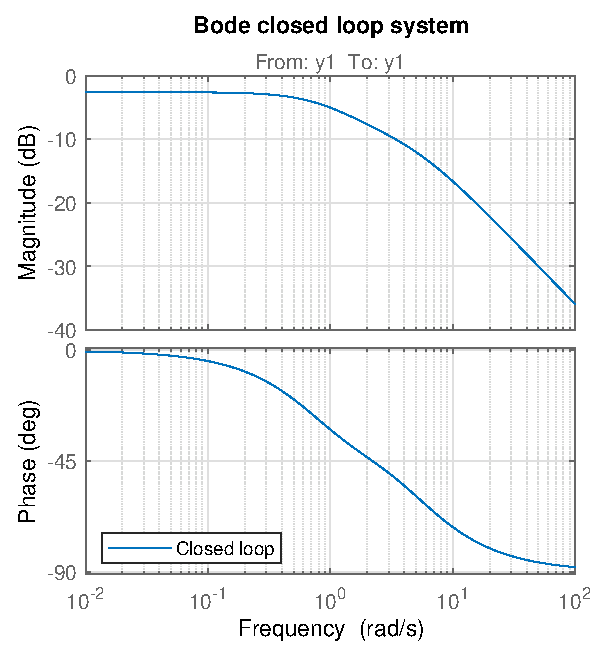
\includegraphics[width=0.9\textwidth]{figures/appendix/bode_closed_loop.eps}
    \caption{Closed loop frequency response (from $\omega_{ref}$ to $\omega_{out}$) of controlled system}
    \label{fig:systemcontrollerbode}
\end{figure}

\begin{figure}[h]
    \centering
    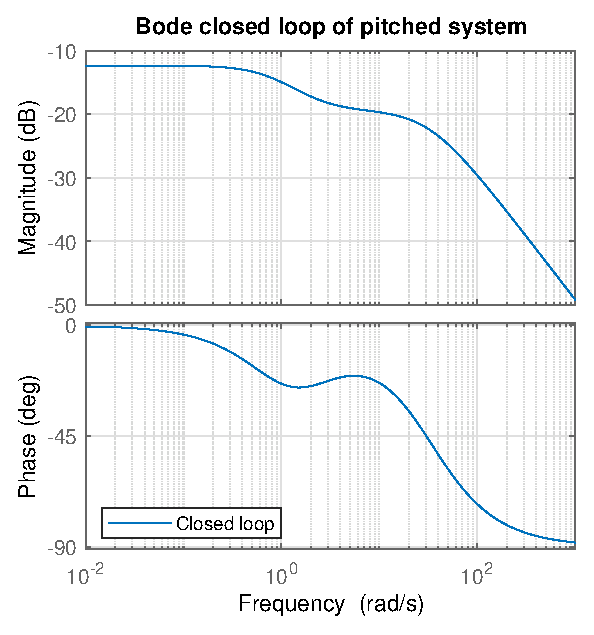
\includegraphics[width=0.9\textwidth]{figures/appendix/bode_closed_loop_pitch.eps}
    \caption{Closed loop frequency response (from $\omega_{ref}$ to $\omega_{out}$) of controlled system with pitched wings}
    \label{fig:systempitchcontrollerbode}
\end{figure}

\begin{sidewaysfigure}
    \centering
    \includegraphics[width=1\textwidth]{figures/system_modelling/top_level_block_diagram.PNG}
    \caption{Top level view of the Simulink model of the drone}
    \label{fig:toplevelmodel}
\end{sidewaysfigure}



\chapter{Video of flight test}
\href{https://youtu.be/Mw67W8S0a4E}{Link} to drone flight test: https://youtu.be/Mw67W8S0a4E\label{link:droneflight}

\chapter{Yaw drift test}
\begin{figure}[h]
    \centering
    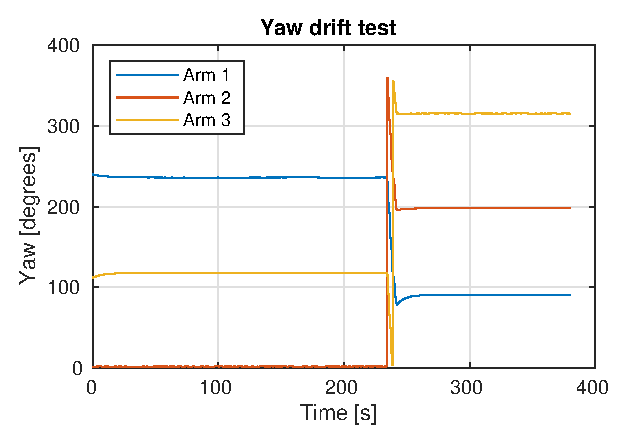
\includegraphics[width=0.9\textwidth]{figures/results/Yaw_drifttest.eps}
    \caption{Test of yaw drift. Measured for approximately 6 minutes. Manually did a rotation of about 170 degrees after 4 minutes}
    \label{fig:yawdrifttest}
\end{figure}

\backmatter
\printbibliography

\cleartoevenpage %To make it look nice.
\include{prefrontmatter/colophon}

\end{document}
